% =============================================================
%  基于非负矩阵分解的神经网络隐藏层表示分析
%  ReLU 与 Tanh 在 MNIST 上的比较研究 —— 实验报告
%  编译：latexmk -xelatex report.tex
% =============================================================
\documentclass[UTF8,a4paper,11pt]{ctexart}

% ---------- 作者信息（请在此处修改） ----------
\newcommand{\InfoAuthor}{作者姓名}
\newcommand{\InfoInstitute}{学校 / 学院}
\newcommand{\InfoDate}{日期}
% ----------------------------------------------

\usepackage[margin=2.5cm]{geometry}
\usepackage{amsmath,amssymb,bm}
\usepackage{graphicx}
\usepackage{booktabs}
\usepackage{multirow}
\usepackage{array}
\usepackage{caption}
\usepackage{subcaption}
\usepackage{xcolor}
\usepackage{tikz}
\usetikzlibrary{arrows.meta,positioning}
\usepackage[numbers,sort&compress]{gbt7714}
\usepackage[colorlinks=true,linkcolor=blue!50!black,citecolor=blue!50!black,urlcolor=blue!50!black]{hyperref}

\graphicspath{{../../figures/}{../../figures/nmf/}}

\definecolor{navy}{HTML}{1F3A5F}
\definecolor{relucol}{HTML}{1F77B4}
\definecolor{tanhcol}{HTML}{FF7F0E}

\ctexset{
  section = {name={第,章},number=\chinese{section},format=\Large\bfseries\color{navy}},
  subsection = {format=\large\bfseries},
}
\captionsetup{font=small,labelsep=quad}
\renewcommand{\arraystretch}{1.15}
\setlength{\parskip}{0.2em}
\setlength{\emergencystretch}{3em}
\setcounter{tocdepth}{1}

\newcommand{\Arelu}{A_{\mathrm{ReLU}}}
\newcommand{\Atanh}{A_{\mathrm{Tanh}}}
\newcommand{\Apos}{A^{+}_{\mathrm{Tanh}}}
\newcommand{\code}[1]{\texttt{\small #1}}

\title{\textbf{基于非负矩阵分解的神经网络隐藏层表示分析}\\[0.3em]
\large ReLU 与 Tanh 在 MNIST 上的比较研究\\[0.6em]
\normalsize Understanding Neural Network Representations through Nonnegative Matrix Factorization:\\
A Comparative Study of ReLU and Tanh on MNIST}
\author{\InfoAuthor\\{\small \InfoInstitute}}
\date{\InfoDate}

\begin{document}
\maketitle

% =============================================================
\begin{abstract}
\noindent
从数值线性代数的角度看，神经网络的隐藏层激活可以作为一个普通矩阵来分析。ReLU 会把负的预激活值截断为零，因此得到的激活矩阵天然非负；这与非负矩阵分解（NMF）的约束在形式上一致。NMF 只允许非负成分相加，常被认为倾向于产生“部分—整体”式的表示。本文以 MNIST 手写数字识别为案例，训练了两个结构相同、仅激活函数不同的单隐藏层全连接网络（784--128--10）。在全部 10000 个测试样本上提取隐藏层激活矩阵后，我们比较了两者的数值分布与稀疏性，并在 8 个秩（$k=4$ 至 $64$）下对 ReLU 激活矩阵和 Tanh 激活矩阵的正值部分分别进行 NMF。

实验观察如下。两个网络的测试准确率分别为 97.13\% 与 96.83\%。ReLU 激活中 38.43\% 的元素恰好为零，按样本计算的平均 Hoyer 稀疏度为 0.396；Tanh 激活呈向 $\pm1$ 两端饱和的 U 形分布。两组矩阵的 NMF 相对重构误差都随秩单调下降；除 $k=4$ 外，ReLU 矩阵的误差均更低。在 $k\le48$ 时，ReLU 分解得到的成分在神经元维度上也更集中，但这一优势随秩增大而缩小，到 $k=64$ 时略有反转。

这些结果说明，在当前设定下，ReLU 激活矩阵更容易被少量非负成分近似。但它们并不能证明 ReLU 表示“更可解释”。本文的局限主要有四点：Tanh 正值部分并非完整的 Tanh 表示；部分 NMF 配置在达到迭代上限时仍未满足收敛条件；每种模型仅训练一次；稀疏性不等于语义可解释性。

\vspace{0.5em}
\noindent\textbf{关键词：}非负矩阵分解；ReLU；Tanh；隐藏层表示；稀疏性；MNIST
\end{abstract}

\newpage
\tableofcontents
\newpage

% =============================================================
\section{引言}

深度神经网络在图像识别等任务上取得了很高的准确率，但其内部如何组织信息往往难以直接解读。对于“可解释性”本身，目前也没有统一的定义和评价标准 \cite{doshivelez2017towards}。一种朴素而可操作的思路，是把网络的中间表示当作数据本身来分析：给定一批输入，某一隐藏层的输出可以排成一个“样本 $\times$ 神经元”的矩阵，矩阵分析的各种工具都可以用在它上面。

在众多矩阵分解方法中，非负矩阵分解（Nonnegative Matrix Factorization, NMF）与本研究的关系最为直接。Lee 与 Seung \cite{lee1999learning} 指出，由于 NMF 的因子均受非负约束，数据只能由若干成分\emph{相加}而成，不允许相互抵消；在人脸图像等数据上，这种约束得到了类似“眼睛”“嘴巴”的局部成分。这一结果常被概括为 NMF 倾向于学习“部分—整体”式表示。另一方面，ReLU 激活函数 \cite{nair2010relu,glorot2011deep} 把负的预激活截断为零，使隐藏层输出非负且常常稀疏。Glorot 等人 \cite{glorot2011deep} 还讨论了这种精确零值稀疏性可能带来的好处。

这两点放在一起，就引出一个直观的问题：ReLU 网络的非负隐藏层激活，是否与 NMF 所偏好的加性、稀疏结构有某种对应？如果有，用 NMF 分解 ReLU 激活矩阵，或许能得到比带符号激活更集中、更有结构的成分。为了让比较有参照，本文选择 Tanh 作为对照。Tanh 的输出有正有负，且两端饱和，在数值性质上与 ReLU 差别明显。

本文的目标是通过数值实验观察上述联系，而不是建立 ReLU 与 NMF 之间的理论等价。具体而言，我们围绕以下五个问题组织实验与讨论：
\begin{enumerate}
  \item ReLU 和 Tanh 是否会产生分布特征不同的隐藏层激活？
  \item ReLU 产生的非负激活是否具有更明显的稀疏性？
  \item 对隐藏层激活矩阵进行 NMF，能否得到权重分布各不相同的成分？
  \item ReLU 激活矩阵与 Tanh 激活矩阵的正值部分，在 NMF 重构误差与分解后稀疏性方面有何差异？
  \item 这些数值实验能在多大程度上帮助我们理解网络内部的表示结构？
\end{enumerate}

本研究的范围限于 MNIST 数据集上的单隐藏层全连接网络，激活矩阵均来自测试集。所有结论都只针对这一具体设定。

% =============================================================
\section{数学背景}

\subsection{ReLU 与 Tanh 激活函数}

设隐藏层的预激活为 $z=W_1x+b_1\in\mathbb{R}^{128}$。两种激活函数逐元素作用：
\begin{equation}
  \mathrm{ReLU}(z)=\max(0,z),\qquad
  \tanh(z)=\frac{e^{z}-e^{-z}}{e^{z}+e^{-z}}.
\end{equation}
二者的差异可以概括为三点。第一是值域：ReLU 的输出在 $[0,\infty)$ 内，Tanh 的输出在 $(-1,1)$ 内。第二是零值：只要 $z\le0$，ReLU 的输出就\emph{恰好}为零，因而会自然产生精确零值；Tanh 只在 $z=0$ 时为零，在浮点运算中几乎不出现精确零值。第三是饱和：Tanh 在 $|z|$ 较大时两端趋于 $\pm1$，导数趋于零；ReLU 只在负半轴上梯度为零，正半轴是线性的。

\subsection{非负矩阵分解}

给定非负矩阵 $A\in\mathbb{R}_{\ge0}^{N\times d}$ 与目标秩 $k<\min(N,d)$，NMF 寻找两个非负因子 $W\in\mathbb{R}_{\ge0}^{N\times k}$ 与 $H\in\mathbb{R}_{\ge0}^{k\times d}$，使 $A\approx WH$。本文使用 Frobenius 范数下的标准形式 \cite{lee2000algorithms}：
\begin{equation}
  \min_{W\ge0,\;H\ge0}\ \frac12\,\|A-WH\|_F^2 .
  \label{eq:nmf}
\end{equation}
该问题对 $W,H$ 联合非凸，一般只能求得局部最优解，结果依赖于初始化与求解器。本文使用 scikit-learn \cite{pedregosa2011sklearn} 的实现：求解器为坐标下降（\code{cd}），属于 Cichocki 与 Phan \cite{cichocki2009fast} 所述的逐块局部更新一类算法；初始化为 \code{nndsvda}，即基于 SVD 的 NNDSVD 方法 \cite{boutsidis2008svd}，零元素用数据均值填充的变体。

\subsection{$W$ 与 $H$ 的含义}

在本文中，$A$ 的每一行 $a_i^\top$ 是第 $i$ 个测试样本的 128 维隐藏层激活。式 \eqref{eq:nmf} 的近似可以逐行写成
\begin{equation}
  a_i \approx \sum_{j=1}^{k} w_{ij}\, h_j ,\qquad w_{ij}\ge0,\ h_j\in\mathbb{R}_{\ge0}^{128},
\end{equation}
其中 $h_j^\top$ 是 $H$ 的第 $j$ 行。因此：
\begin{itemize}
  \item $H$ 的每一行是\textbf{神经元空间中的一个成分}（component），描述哪些隐藏神经元倾向于一同被激活；
  \item $W$ 的第 $i$ 行是样本 $i$ 在 $k$ 个成分上的\textbf{非负系数}。
\end{itemize}
由于所有系数和成分都非负，每个样本的激活只能由成分\emph{叠加}得到，成分之间不能相互抵消。这正是 NMF 常被认为倾向产生局部表示的直觉来源 \cite{lee1999learning}。需要注意，本文的矩阵是“样本 $\times$ 特征”排列，与 Lee 和 Seung 论文中“特征 $\times$ 样本”的排列互为转置，因此这里的 $H$ 对应原文中的“基”。

\subsection{相对重构误差}

为了在不同尺度的矩阵之间比较近似质量，本文使用相对 Frobenius 误差
\begin{equation}
  \varepsilon_k=\frac{\|A-WH\|_F}{\|A\|_F}.
\end{equation}
$\varepsilon_k$ 越小，说明 $A$ 越能被 $k$ 个非负成分近似。它衡量的是“低秩非负可近似性”，与成分是否具有语义无直接关系。

\subsection{Hoyer 稀疏度}

对于非零向量 $x\in\mathbb{R}^n$，Hoyer \cite{hoyer2004nmf} 定义的稀疏度为
\begin{equation}
  S(x)=\frac{\sqrt{n}-\|x\|_1/\|x\|_2}{\sqrt{n}-1}\in[0,1].
  \label{eq:hoyer}
\end{equation}
由 Cauchy--Schwarz 不等式，$\|x\|_2\le\|x\|_1\le\sqrt n\,\|x\|_2$。当 $x$ 只有一个非零元时 $S=1$；当所有元素的绝对值相等时 $S=0$。$S$ 对缩放不变，衡量的是\textbf{幅度在各维度上的集中程度}，而不是零元素的个数。本文在两处使用该指标：
\begin{itemize}
  \item \textbf{原始激活}：对 $A$ 的每一行（每个样本，$n=128$）计算 $S$ 后取平均；对 Tanh 使用 $|a|$。
  \item \textbf{NMF 成分}：对 $H$ 的每一行（每个成分，$n=128$）计算 $S$ 后取平均。
\end{itemize}
这两种稀疏度的对象不同，前者描述网络激活本身，后者描述分解得到的成分，下文不会混用。

% =============================================================
\section{实验设计与实现}

本章所述的配置均取自仓库中的实际代码（\code{src/mnist\_nmf/models.py} 与 \code{scripts/} 下各脚本），未作任何假设。

\subsection{数据集}

实验使用 MNIST 手写数字数据集 \cite{lecun1998gradient}：训练集 60000 张、测试集 10000 张，每张为 $28\times28$ 灰度图像，共 10 个类别。预处理仅为 \code{transforms.ToTensor()}，即把像素值缩放到 $[0,1]$，没有做均值—方差标准化或数据增强。测试集的类别分布为：数字 0--9 各有 980、1135、1032、1010、982、892、958、1028、974、1009 个样本。图 \ref{fig:mnist} 给出了若干训练样本。

\begin{figure}[htbp]
  \centering
  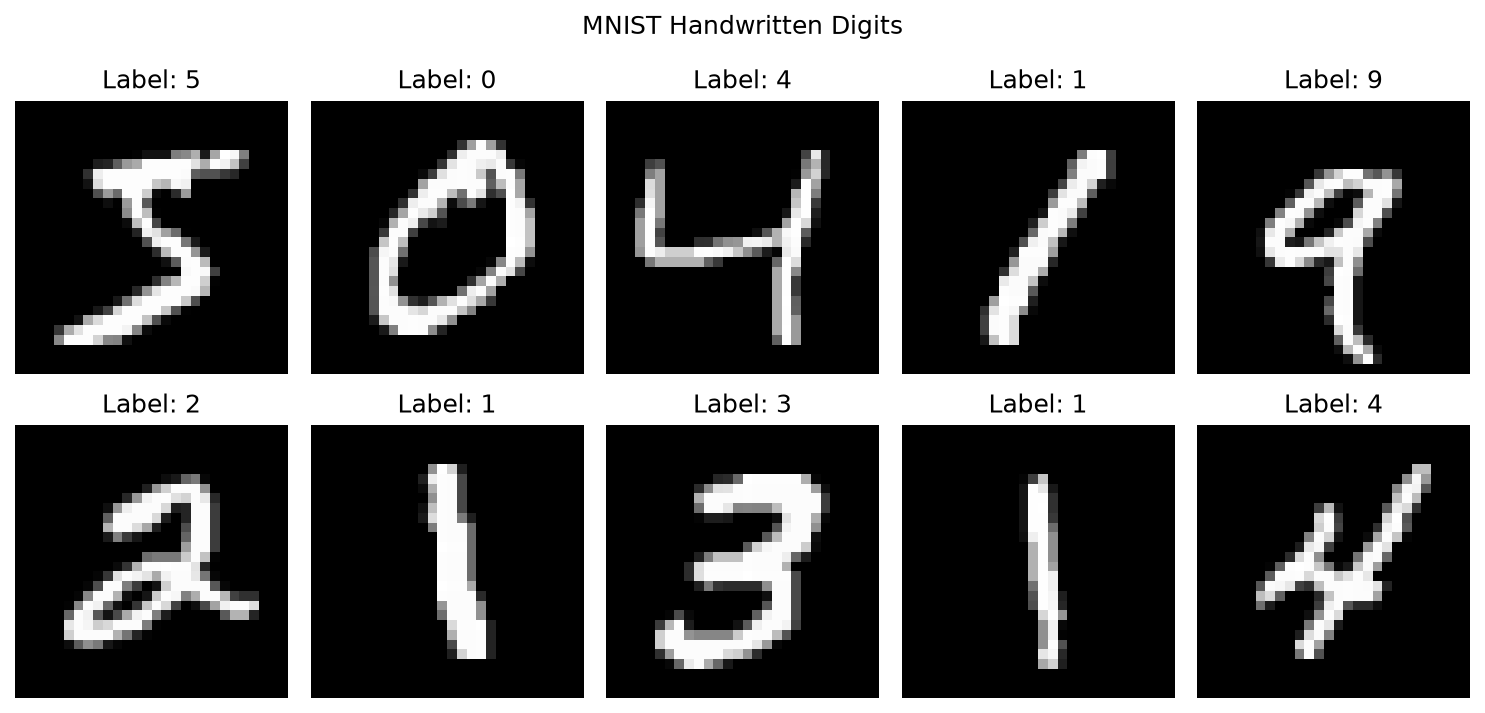
\includegraphics[width=0.62\textwidth]{mnist_samples.png}
  \caption{MNIST 训练集中的前 10 个样本（\code{reports/figures/mnist\_samples.png}）。}
  \label{fig:mnist}
\end{figure}

\subsection{网络结构}

两个模型均为单隐藏层多层感知机 \code{MNISTMLP}，结构如图 \ref{fig:arch} 所示：输入图像先展平为 784 维向量，经全连接层映射到 128 维，再经激活函数（ReLU 或 Tanh），最后由全连接层输出 10 维 logits。两个模型的可训练参数均为
\[
  (784\times128+128)+(128\times10+10)=100480+1290=101770 .
\]
隐藏层激活通过 \code{forward\_features} 方法提取，即激活函数的输出 $h=\sigma(W_1x+b_1)$。

\begin{figure}[htbp]
\centering
\begin{tikzpicture}[
  font=\small,
  lay/.style={draw=navy,rounded corners=2pt,minimum height=1.0cm,align=center,line width=0.7pt},
  arr/.style={-{Stealth[length=2mm]},line width=0.8pt,navy}]
  \node[lay] (in) {输入\\$1\times28\times28$};
  \node[lay,right=0.5cm of in] (fl) {Flatten\\784};
  \node[lay,right=0.5cm of fl] (fc1) {Linear\\$784\to128$};
  \node[lay,right=0.5cm of fc1,fill=navy!8,minimum width=1.8cm] (act) {\textcolor{relucol}{\textbf{ReLU}} 或\\\textcolor{tanhcol}{\textbf{Tanh}}};
  \node[lay,right=0.5cm of act] (fc2) {Linear\\$128\to10$};
  \draw[arr] (in)--(fl); \draw[arr] (fl)--(fc1); \draw[arr] (fc1)--(act); \draw[arr] (act)--(fc2);
  \node[draw=tanhcol!80!black,dashed,rounded corners=2pt,below=0.6cm of act,align=center,font=\footnotesize] (A)
       {隐藏层激活矩阵 $A\in\mathbb{R}^{10000\times128}$};
  \draw[arr,dashed] (act)--(A);
\end{tikzpicture}
\caption{网络结构与激活提取位置。两个模型唯一的区别是隐藏层激活函数。}
\label{fig:arch}
\end{figure}

\subsection{训练配置}

训练脚本为 \code{scripts/train\_models.py}，配置见表 \ref{tab:config}。为了使对照尽量公平，脚本先以种子 42 构造一个模型，并把它的初始权重复制给 ReLU 和 Tanh 两个模型；训练前重置随机种子，并为 \code{DataLoader} 指定同一个随机生成器，使两次训练的数据顺序一致。因此，两个模型的差异仅来自激活函数，以及由此引起的不同优化轨迹。每个 epoch 结束后在测试集上评估一次。

\begin{table}[htbp]
  \centering
  \caption{模型与训练配置（取自 \code{train\_models.py}）}
  \label{tab:config}
  \begin{tabular}{ll}
    \toprule
    项目 & 设置 \\
    \midrule
    网络结构 & 784 -- 128 -- 10，单隐藏层 MLP \\
    参数量 & 101{,}770 \\
    损失函数 & 交叉熵（\code{nn.CrossEntropyLoss}） \\
    优化器 & Adam \cite{kingma2015adam}，学习率 $1\times10^{-3}$，其余为 PyTorch 默认值 \\
    批大小 / 训练轮数 & 128 / 5 epochs \\
    随机种子 & 42（两个模型共享初始权重与数据顺序） \\
    运行设备 & 代码自动选择 CUDA 或 CPU；本次运行的设备未记录 \\
    \bottomrule
  \end{tabular}
\end{table}

\subsection{激活提取}

训练结束后，脚本 \code{scripts/extract\_activations.py} 载入两个模型，在全部 10000 个测试样本上（不打乱顺序）提取隐藏层输出，得到 $\Arelu,\Atanh\in\mathbb{R}^{10000\times128}$ 及对应标签。两个矩阵的行一一对应同一测试样本，标签一致性已在后续脚本中用断言检查。

\subsection{NMF 分解流程}

\textbf{ReLU。}$\Arelu$ 本身非负，直接作为 NMF 的输入（\code{scripts/run\_nmf.py}）。

\textbf{Tanh Positive。}$\Atanh$ 含负值，不能直接用于 NMF。脚本 \code{scripts/\allowbreak compare\_relu\_tanh\_nmf.py} 先取其正值部分
\begin{equation}
  \Apos=\max(\Atanh,0),
\end{equation}
再进行分解。必须强调，这一处理把 $\Atanh$ 中全部负值（占 52.16\%）置为零，丢弃了带符号表示的另一半信息。因此下文所说的“Tanh Positive”指 Tanh 激活矩阵的\textbf{正值部分}，而不是完整的 Tanh 表示。由于这一置零，$\Apos$ 中零元素的比例（52.16\%）反而高于 $\Arelu$（38.43\%）。

\textbf{参数设置。}两组实验采用完全相同的设置：秩 $k\in\{4,8,12,16,24,32,48,64\}$，初始化 \code{nndsvda}，求解器 \code{cd}，最大迭代次数 500，随机种子 42，其余参数取 scikit-learn 默认值（收敛容差 \code{tol}$=10^{-4}$，无正则项）。选取的秩从远小于神经元数的 4 一直到神经元数的一半 64，用于观察近似质量随秩的变化趋势。

\textbf{后续分析。}对 ReLU 的 $k=16$ 与 $k=32$ 结果，脚本 \code{visualize\_nmf\_components.py} 绘制了 $H$ 的热力图（每行按行和归一化），并计算了 $H$ 各行的 Hoyer 稀疏度；脚本 \code{analyze\_nmf\_\allowbreak class\_activation.py} 按数字类别计算 $W$ 的类均值，并按成分（列）最大值归一化后绘制热力图。

\subsection{评价指标}

\begin{itemize}
  \item \textbf{分类性能}：测试准确率与平均交叉熵损失。
  \item \textbf{原始激活}：均值、标准差、极值、负值比例、精确零值比例 $\Pr[a=0]$、近零比例 $\Pr[|a|<0.1]$、平均 $|a|$ 以及按样本的平均 Hoyer 稀疏度。
  \item \textbf{神经元层面}：ReLU 每个神经元的零值比例；Tanh 每个神经元的饱和比例 $\Pr[|a|>0.95]$ 与 $\Pr[|a|>0.99]$；类别选择性 $\eta^2$，即类间平方和与总平方和之比（单因素方差分析意义下的效应量）。
  \item \textbf{NMF}：相对重构误差 $\varepsilon_k$、实际迭代次数、$H$ 各行的平均 Hoyer 稀疏度。
\end{itemize}

\textbf{数据来源说明。}大部分数值直接读自 \code{reports/metrics/} 与 \code{reports/activations/} 中的 JSON 文件。其中近零比例 $\Pr[|a|<0.1]$、平均 $|a|$、原始激活的 Hoyer 稀疏度、除 $k=32$ 外各秩下 $H$ 的 Hoyer 稀疏度，以及 \S\ref{sec:class} 中的类别关联统计，仓库中没有对应的指标文件。这些数值是本文撰写时直接从已保存的 \code{reports/activations/*.npz} 与 \code{reports/nmf/*.npz} 计算得到的，没有重新训练模型或重新运行 NMF。另外，\code{activation\_statistics.json} 中的 \code{near\_zero\_ratio} 字段使用的阈值是 $10^{-3}$，与本文表 \ref{tab:act} 中的 $0.1$ 不同。

% =============================================================
\section{实验结果}

\subsection{分类性能}

表 \ref{tab:cls} 给出两个模型第 5 个 epoch 结束时的结果。二者测试准确率都在 97\% 左右，ReLU 高出 0.30 个百分点，测试损失也略低。从每个 epoch 的记录看（\code{training\_results.json}），ReLU 在全部 5 个 epoch 中的测试准确率都略高于 Tanh，差距在 0.3--0.5 个百分点之间。

\begin{table}[htbp]
  \centering
  \caption{分类性能（第 5 个 epoch；\code{reports/metrics/training\_results.json}）}
  \label{tab:cls}
  \begin{tabular}{lrr}
    \toprule
    指标 & \textcolor{relucol}{ReLU} & \textcolor{tanhcol}{Tanh} \\
    \midrule
    测试准确率 & 0.9713 & 0.9683 \\
    测试损失 & 0.0955 & 0.1070 \\
    训练损失 & 0.0845 & 0.0944 \\
    训练时间（秒） & 38.57 & 39.22 \\
    \bottomrule
  \end{tabular}
\end{table}

需要说明两点：每个模型只训练了一次，没有不同随机种子下的方差估计，因此这一差距不能被视为统计显著；训练时间包含每轮测试评估，且运行设备未记录，仅供参考。对本文而言，这一结果的主要意义在于说明\textbf{两个模型都已经学到了有效的分类表示}，后续对隐藏层的比较是在两个性能相近的网络之间进行的。

\subsection{原始激活分布}

图 \ref{fig:dist} 展示了两组激活值的整体分布，表 \ref{tab:act} 汇总了主要统计量。

\begin{figure}[htbp]
  \centering
  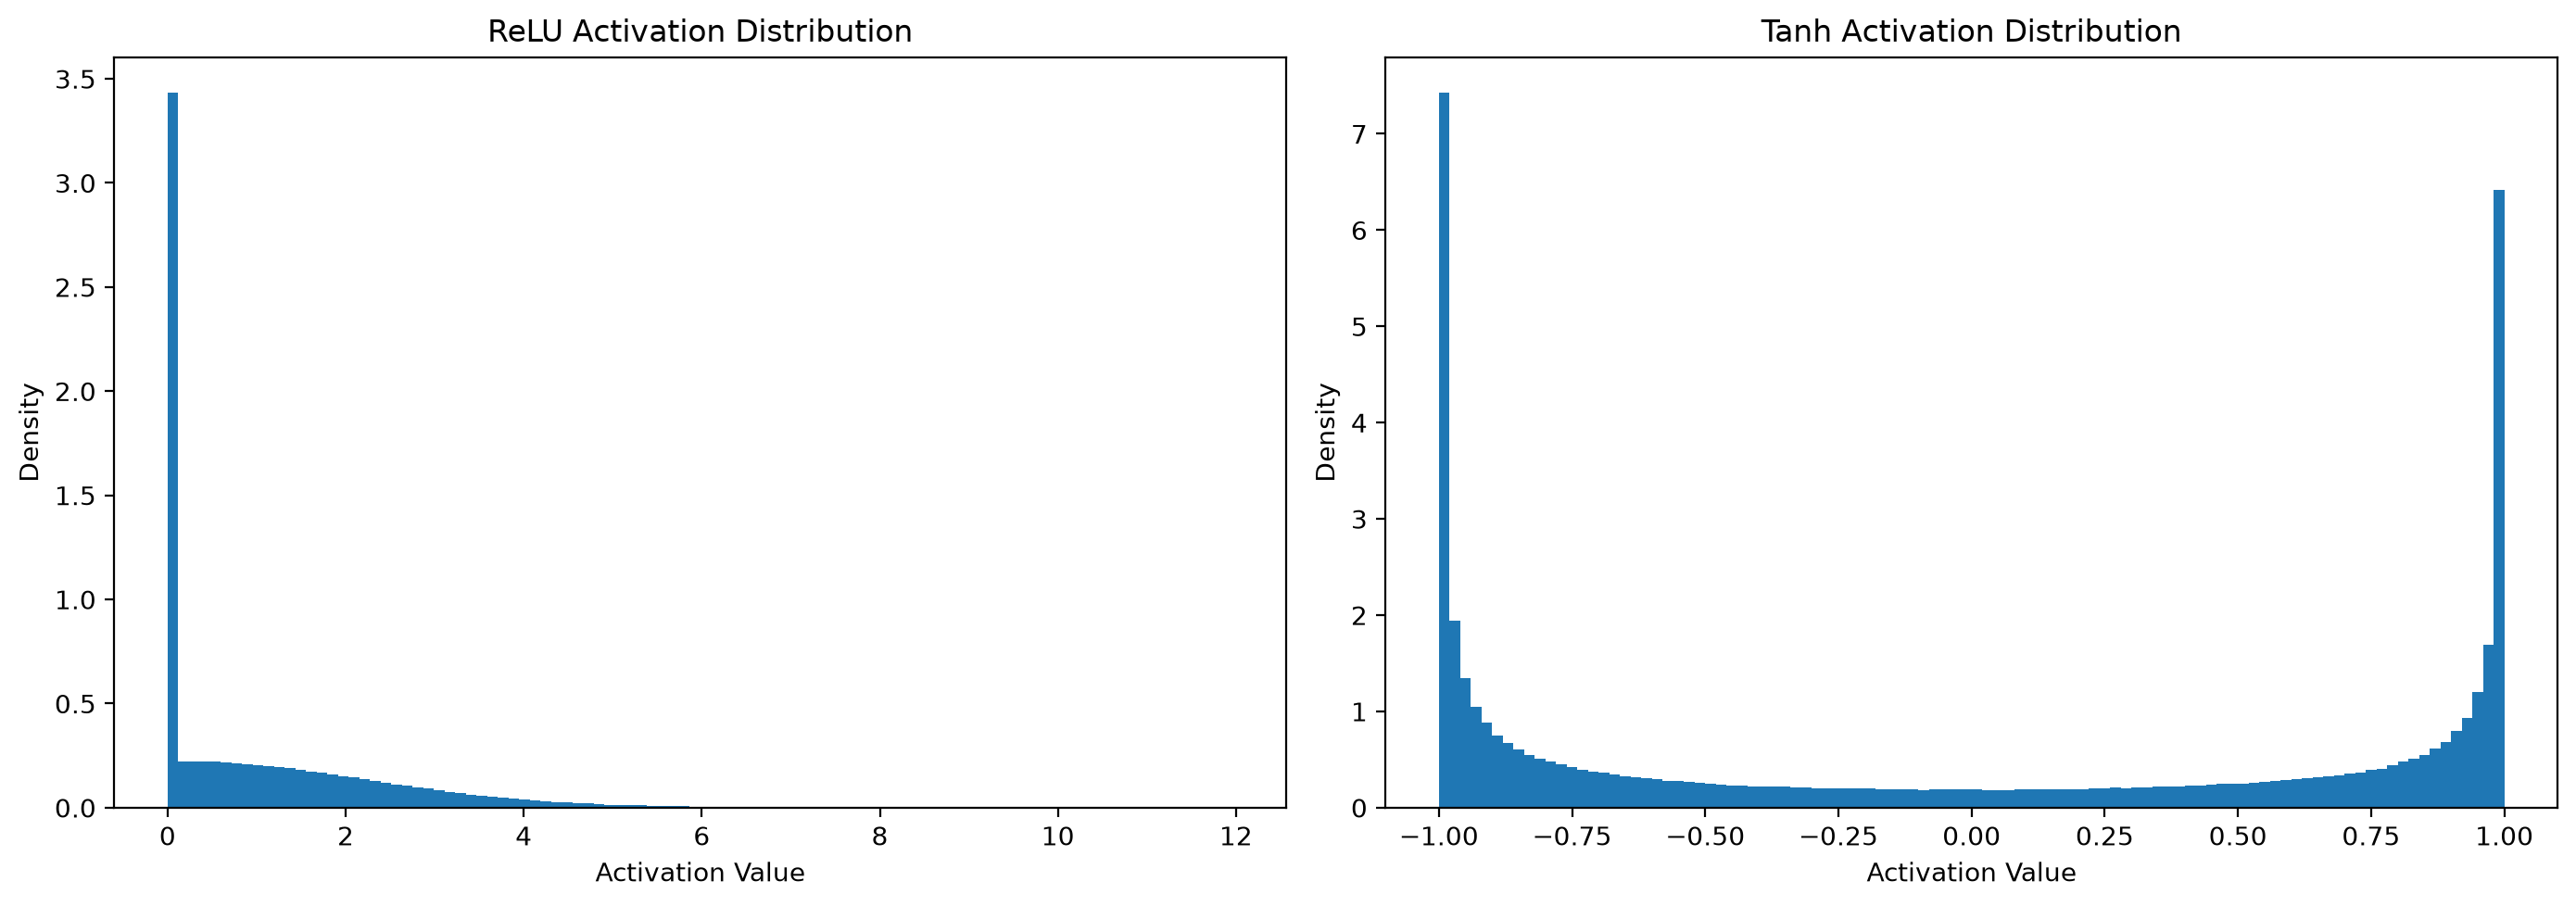
\includegraphics[width=\textwidth]{activation_distributions.png}
  \caption{全部 $10000\times128$ 个隐藏层激活值的分布（密度直方图，100 个分箱）。左：ReLU；右：Tanh。（\code{reports/figures/activation\_distributions.png}）}
  \label{fig:dist}
\end{figure}

ReLU 的分布在零点处有一个很高的尖峰，对应 38.43\% 恰好为零的激活。其余激活为正值，构成一个右偏的长尾，大部分在 0 到 6 之间，最大值为 11.97。Tanh 的分布则近似对称（均值 $-0.040$），呈 U 形：大量激活集中在 $-1$ 和 $+1$ 附近，中间区域密度较低。按神经元统计（\code{neuron\_summary.json}），Tanh 神经元平均有 37.7\% 的激活满足 $|a|>0.95$，21.9\% 满足 $|a|>0.99$。也就是说，相当一部分 Tanh 激活工作在饱和区，表现得接近二值的 $\pm1$ 信号。

\begin{figure}[htbp]
  \centering
  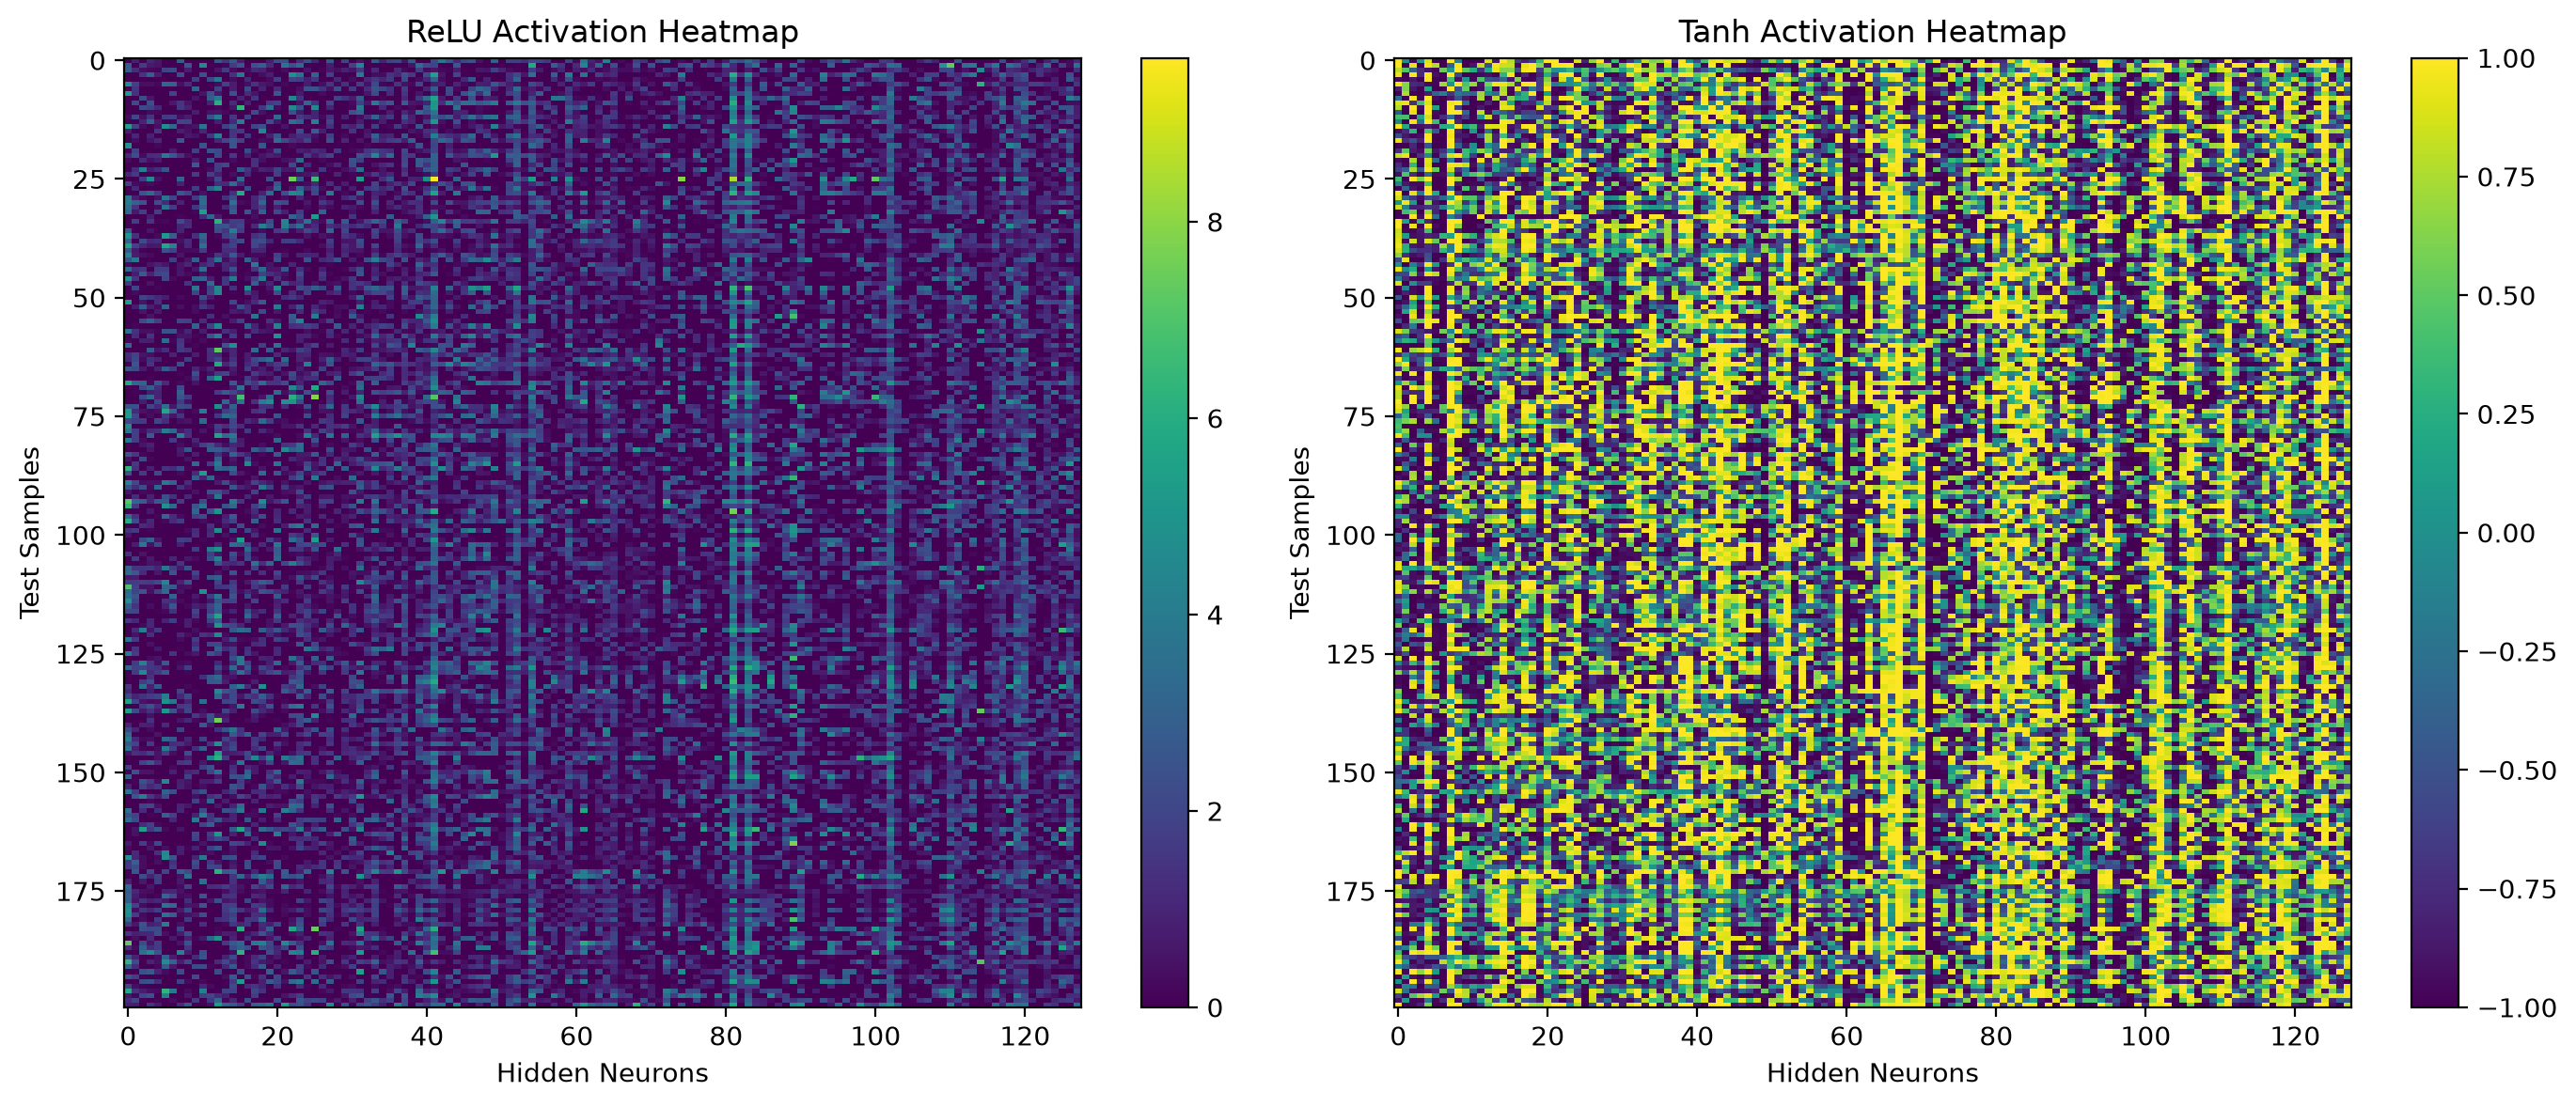
\includegraphics[width=\textwidth]{activation_heatmaps.png}
  \caption{前 200 个测试样本的激活热力图（行：样本，列：隐藏神经元）。左：ReLU（色标 $[0,\approx9.6]$）；右：Tanh（色标 $[-1,1]$）。两图色标不同，只宜分别观察。（\code{reports/figures/activation\_heatmaps.png}）}
  \label{fig:heat}
\end{figure}

图 \ref{fig:heat} 从样本层面展示了同样的差异。ReLU 热力图以深色（零或小值）为主，少数神经元列（如编号 80 附近与 100 附近）在多数样本上持续取较大值。Tanh 热力图则在两种极端颜色之间频繁切换，几乎没有“静默”的元素。

\subsection{原始激活稀疏性}

\begin{table}[htbp]
  \centering
  \caption{原始隐藏层激活的统计量（$10000\times128$）。带 $^\dagger$ 的数值由 \code{reports/activations/*.npz} 计算，其余取自 \code{activation\_statistics.json}。}
  \label{tab:act}
  \begin{tabular}{lrr}
    \toprule
    指标 & \textcolor{relucol}{ReLU} & \textcolor{tanhcol}{Tanh} \\
    \midrule
    最小值 / 最大值 & 0 / 11.9665 & $-1$ / 1 \\
    均值 & 1.0615 & $-0.0398$ \\
    标准差 & 1.3272 & 0.8029 \\
    负值比例 & 0 & 0.5216 \\
    精确零值比例 $\Pr[a=0]$ & 0.3843 & 0 \\
    近零比例 $\Pr[|a|<0.1]^\dagger$ & 0.4063 & 0.0376 \\
    平均 $|a|^\dagger$ & 1.0615 & 0.7510 \\
    平均 Hoyer 稀疏度（按样本）$^\dagger$ & 0.3960 & 0.0707 \\
    \bottomrule
  \end{tabular}
\end{table}

表 \ref{tab:act} 从三个角度描述了稀疏性。\textbf{精确零值}方面，ReLU 有 38.43\% 的元素为零，相当于每个样本平均约有 78.8 个神经元处于激活状态；Tanh 没有精确零值。\textbf{近零值}方面，ReLU 中 $|a|<0.1$ 的比例为 40.63\%，只比精确零值高约 2 个百分点，说明 ReLU 激活要么为零，要么明显大于零，介于二者之间的很少；Tanh 中这一比例仅为 3.76\%。\textbf{Hoyer 稀疏度}方面，ReLU 为 0.396，Tanh（基于 $|a|$）仅为 0.071。

对 Tanh 的 Hoyer 值需要谨慎解读。式 \eqref{eq:hoyer} 衡量的是幅度在 128 个维度上分布得是否均匀。Tanh 的大量激活饱和在 $|a|\approx1$ 附近，幅度彼此接近，所以 Hoyer 值很低。这反映的是“幅度均匀”，并不意味着 Tanh 激活中存在零值；而且符号所携带的信息在 $|a|$ 中已经丢失。

\begin{figure}[htbp]
  \centering
  \begin{subfigure}[b]{0.49\textwidth}
    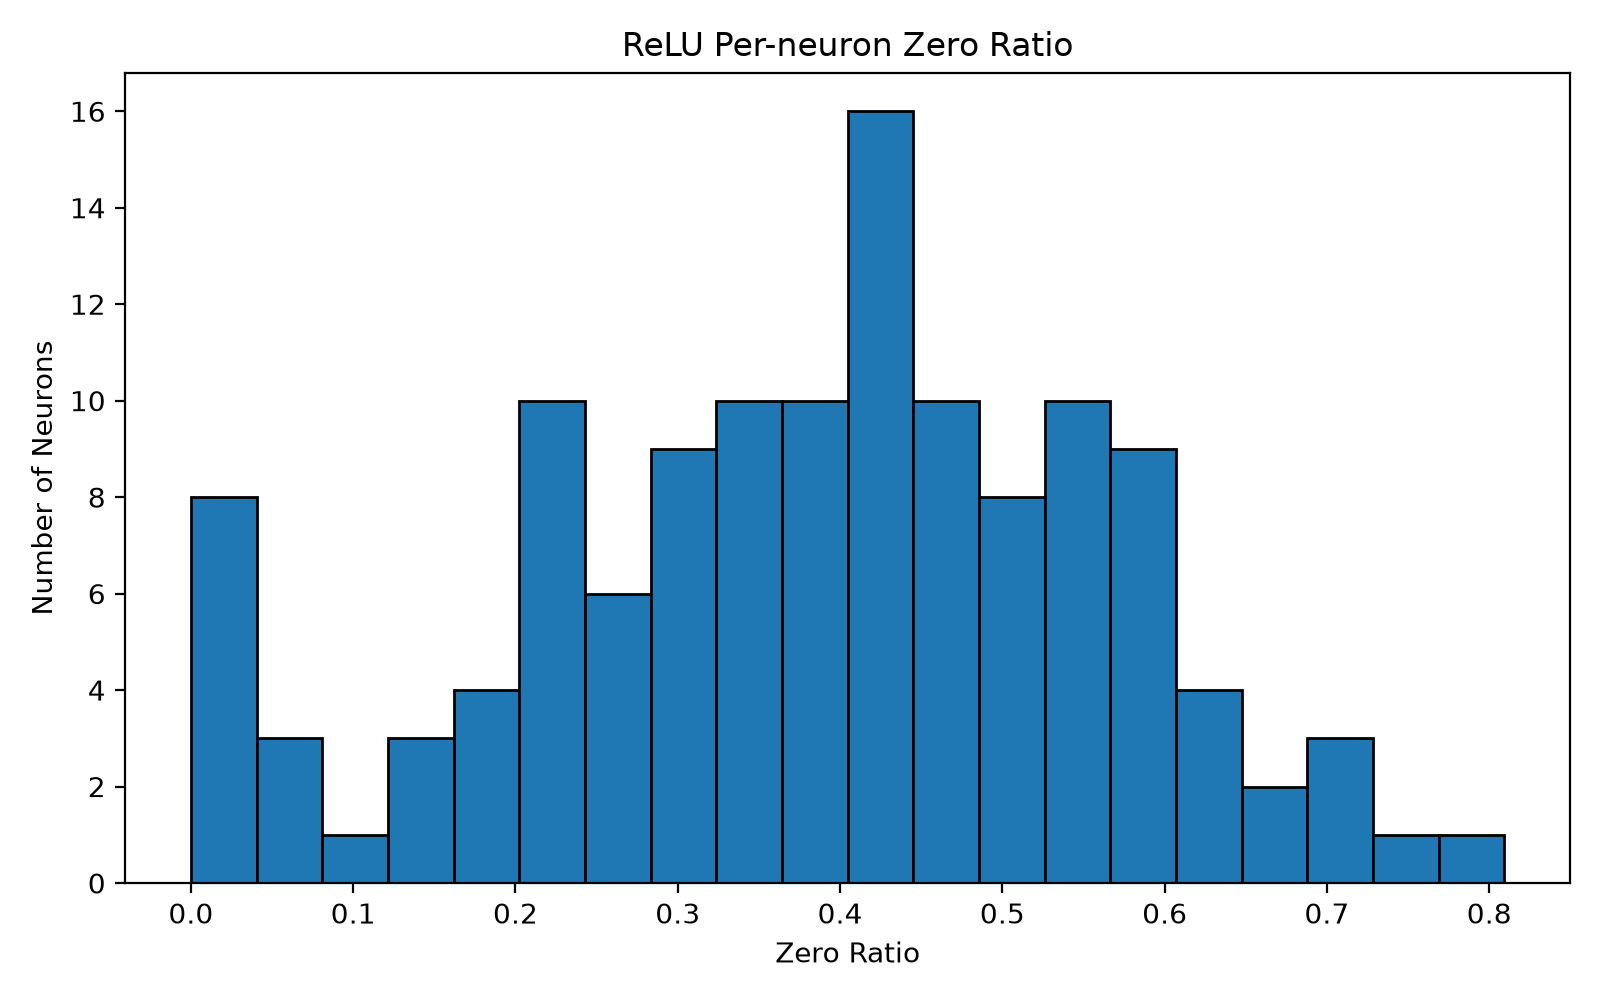
\includegraphics[width=\textwidth]{relu_neuron_sparsity.png}
    \caption{ReLU：每个神经元的零值比例}
  \end{subfigure}\hfill
  \begin{subfigure}[b]{0.49\textwidth}
    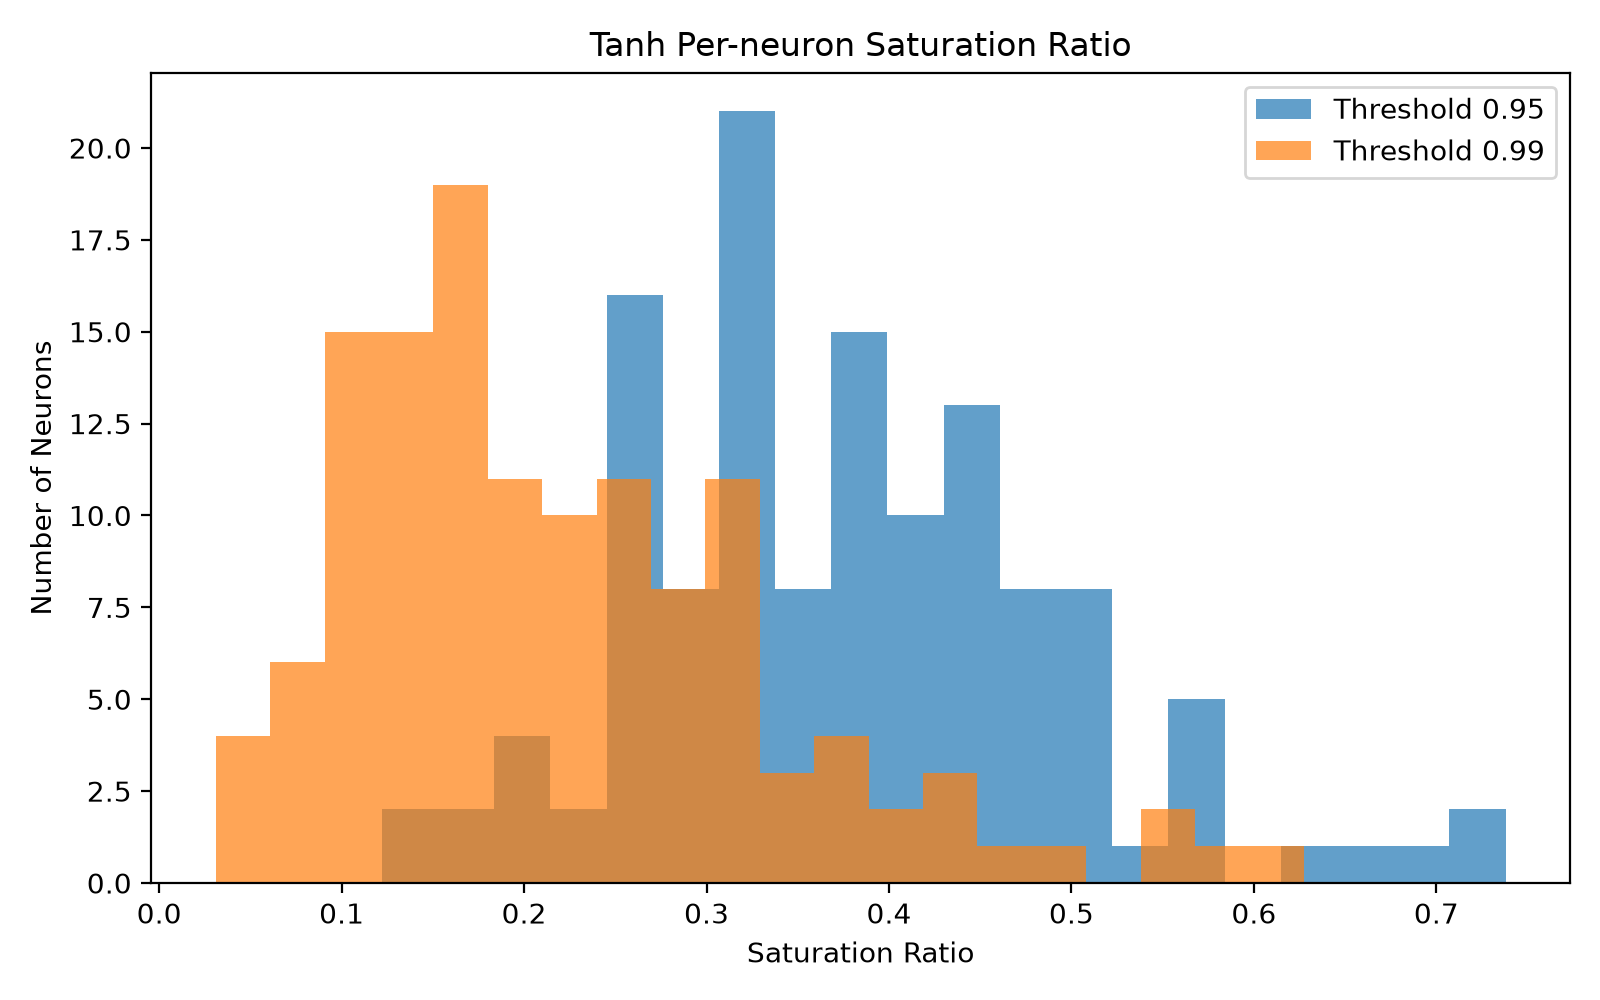
\includegraphics[width=\textwidth]{tanh_neuron_saturation.png}
    \caption{Tanh：每个神经元的饱和比例}
  \end{subfigure}
  \caption{神经元层面的稀疏性与饱和性（128 个神经元的直方图）。图片位于 \code{reports/figures/}。}
  \label{fig:neuron}
\end{figure}

图 \ref{fig:neuron} 把视角转到单个神经元。ReLU 神经元的零值比例差异很大：从 0（有 2 个神经元在所有测试样本上都为正）到 0.81，中位数为 0.40，标准差为 0.18；没有神经元在全部样本上都为零，即不存在“死亡”神经元。Tanh 神经元的饱和比例同样差异明显，阈值 0.95 下为 0.12 到 0.74。因此，两种网络的整体统计量都掩盖了神经元之间相当大的差异。

\begin{figure}[htbp]
  \centering
  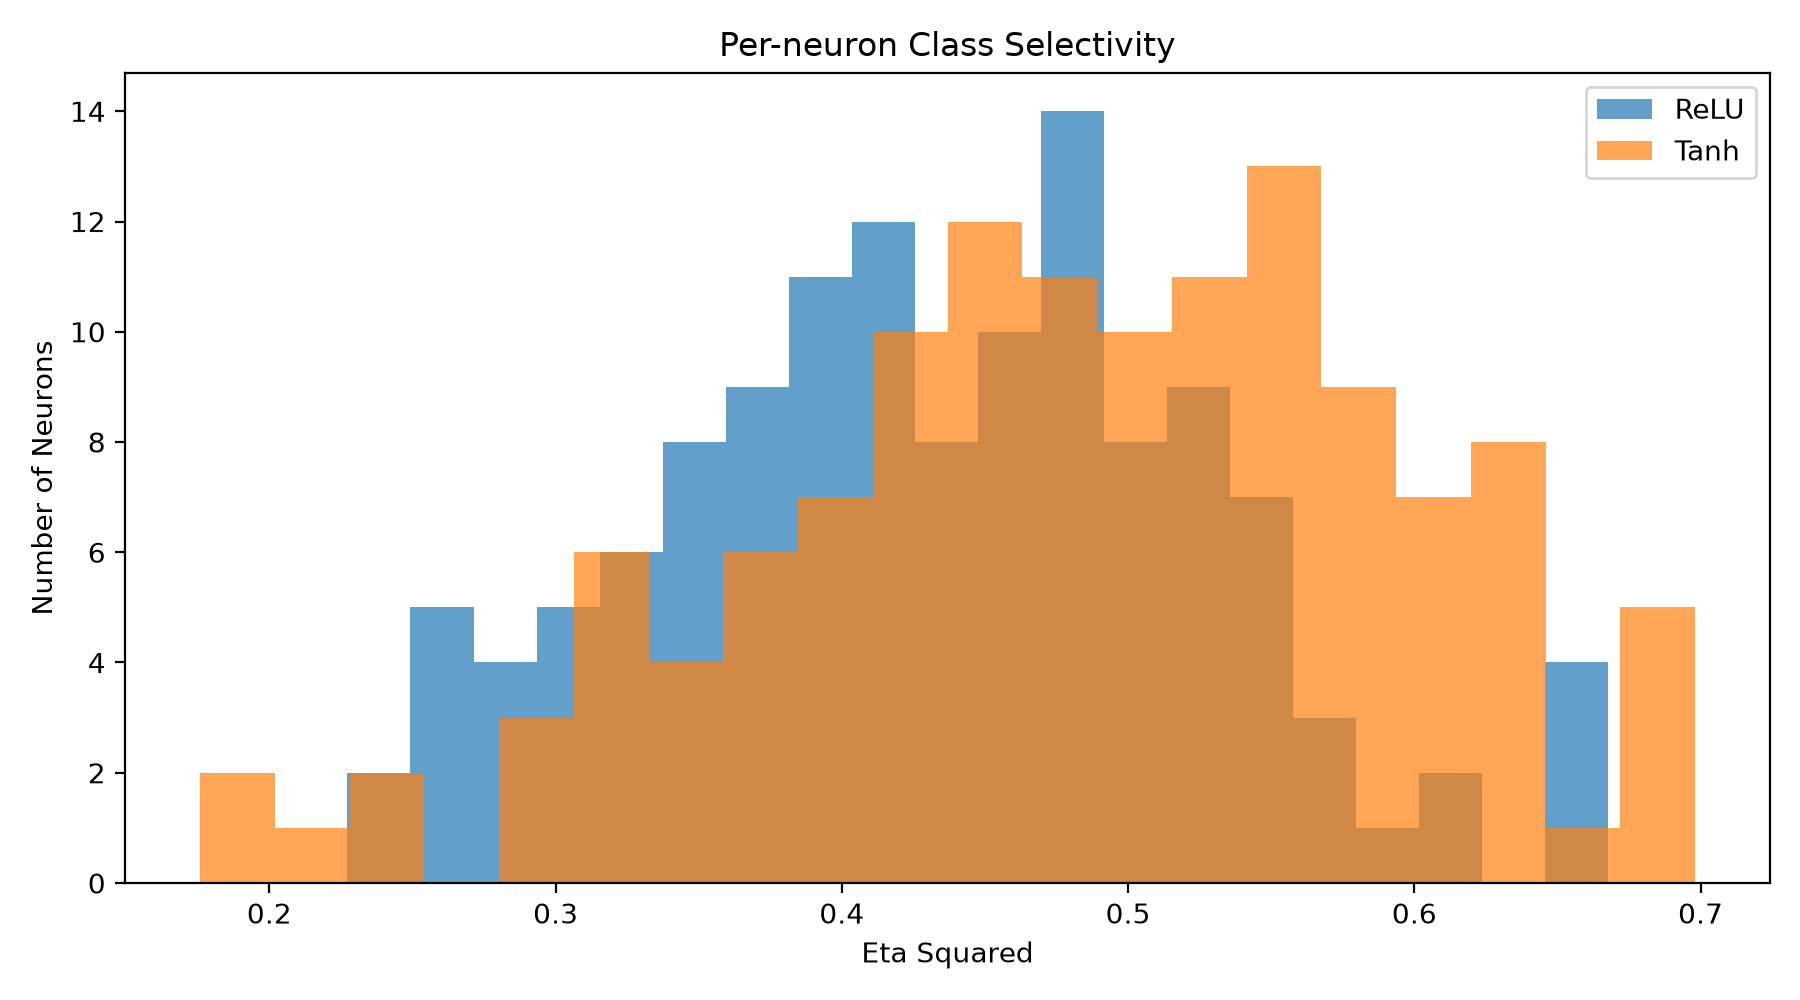
\includegraphics[width=0.72\textwidth]{neuron_class_selectivity.png}
  \caption{各隐藏神经元的类别选择性 $\eta^2$ 分布。（\code{reports/figures/neuron\_class\_selectivity.png}）}
  \label{fig:eta}
\end{figure}

图 \ref{fig:eta} 比较了单个神经元的类别选择性 $\eta^2$。两个分布大幅重叠，Tanh 略偏向高值：平均 $\eta^2$ 为 0.482，ReLU 为 0.433；最大值分别为 0.698 与 0.668。在 ReLU 网络内部，神经元零值比例与 $\eta^2$ 的相关系数仅为 $-0.09$。这两点都说明，在本实验中，\textbf{更稀疏的激活并没有伴随更强的单神经元类别选择性}。

\subsection{NMF 重构误差}

表 \ref{tab:nmf} 列出了各秩下的相对重构误差与实际迭代次数。

\begin{table}[htbp]
  \centering
  \caption{NMF 相对重构误差与迭代次数。误差较低者、以及迭代次数达到上限 500 者加粗。数据来自 \code{reports/metrics/} 下的 \code{nmf\_rank\_comparison.json} 与 \code{tanh\_positive\_nmf\_results.json}。}
  \label{tab:nmf}
  \begin{tabular}{r rr rr}
    \toprule
    \multirow{2}{*}{秩 $k$} & \multicolumn{2}{c}{相对重构误差 $\varepsilon_k$} & \multicolumn{2}{c}{迭代次数} \\
    \cmidrule(lr){2-3}\cmidrule(lr){4-5}
     & \textcolor{relucol}{ReLU} & \textcolor{tanhcol}{Tanh Positive} & ReLU & Tanh Positive \\
    \midrule
     4 & 0.5199 & \textbf{0.5166} & 60 & 69 \\
     8 & \textbf{0.4223} & 0.4442 & 200 & 162 \\
    12 & \textbf{0.3704} & 0.4076 & 316 & \textbf{500} \\
    16 & \textbf{0.3331} & 0.3833 & 258 & 264 \\
    24 & \textbf{0.2830} & 0.3498 & 403 & \textbf{500} \\
    32 & \textbf{0.2458} & 0.3236 & \textbf{500} & \textbf{500} \\
    48 & \textbf{0.1944} & 0.2817 & 439 & \textbf{500} \\
    64 & \textbf{0.1552} & 0.2426 & \textbf{500} & \textbf{500} \\
    \bottomrule
  \end{tabular}
\end{table}

两组误差都随秩单调下降，符合预期：成分越多，近似越精细。两者的相对关系可以分为两段。在 $k=4$ 时，Tanh Positive 的误差略低（0.5166 对 0.5199，相差 0.003）。从 $k=8$ 开始，ReLU 的误差始终更低，且差距随秩增大而扩大：$k=8$ 时相差 0.022，$k=64$ 时相差 0.087。换一种方式看，ReLU 在 $k=16$ 时的误差（0.333）已经与 Tanh Positive 在 $k=32$ 时的误差（0.324）相当，即达到相近的近似质量，ReLU 只需要约一半的成分。

\textbf{收敛情况。}16 组配置中有 7 组的实际迭代次数等于上限 500：ReLU 的 $k=32,64$，以及 Tanh Positive 的 $k=12,24,32,48,64$。scikit-learn 在达到 \code{max\_iter} 仍未满足收敛容差时会发出 \code{ConvergenceWarning}。仓库中没有保存运行日志，因此我们只能从迭代次数推断这 7 组配置未满足收敛条件，无法确认具体的警告信息。未收敛的配置更多出现在 Tanh Positive 一侧，所以其误差可能被略微高估；但在 $k=16$ 这种两组都正常收敛的配置下，ReLU 的误差同样明显更低（0.333 对 0.383），说明 ReLU 的优势并非完全由收敛问题造成。

\subsection{NMF 成分的结构}

图 \ref{fig:comp} 展示了 ReLU 激活矩阵在 $k=16$ 时得到的成分矩阵 $H$。每一行是一个成分，每一列是一个隐藏神经元；为了消除成分之间的整体尺度差异，每一行都按行和归一化。

\begin{figure}[htbp]
  \centering
  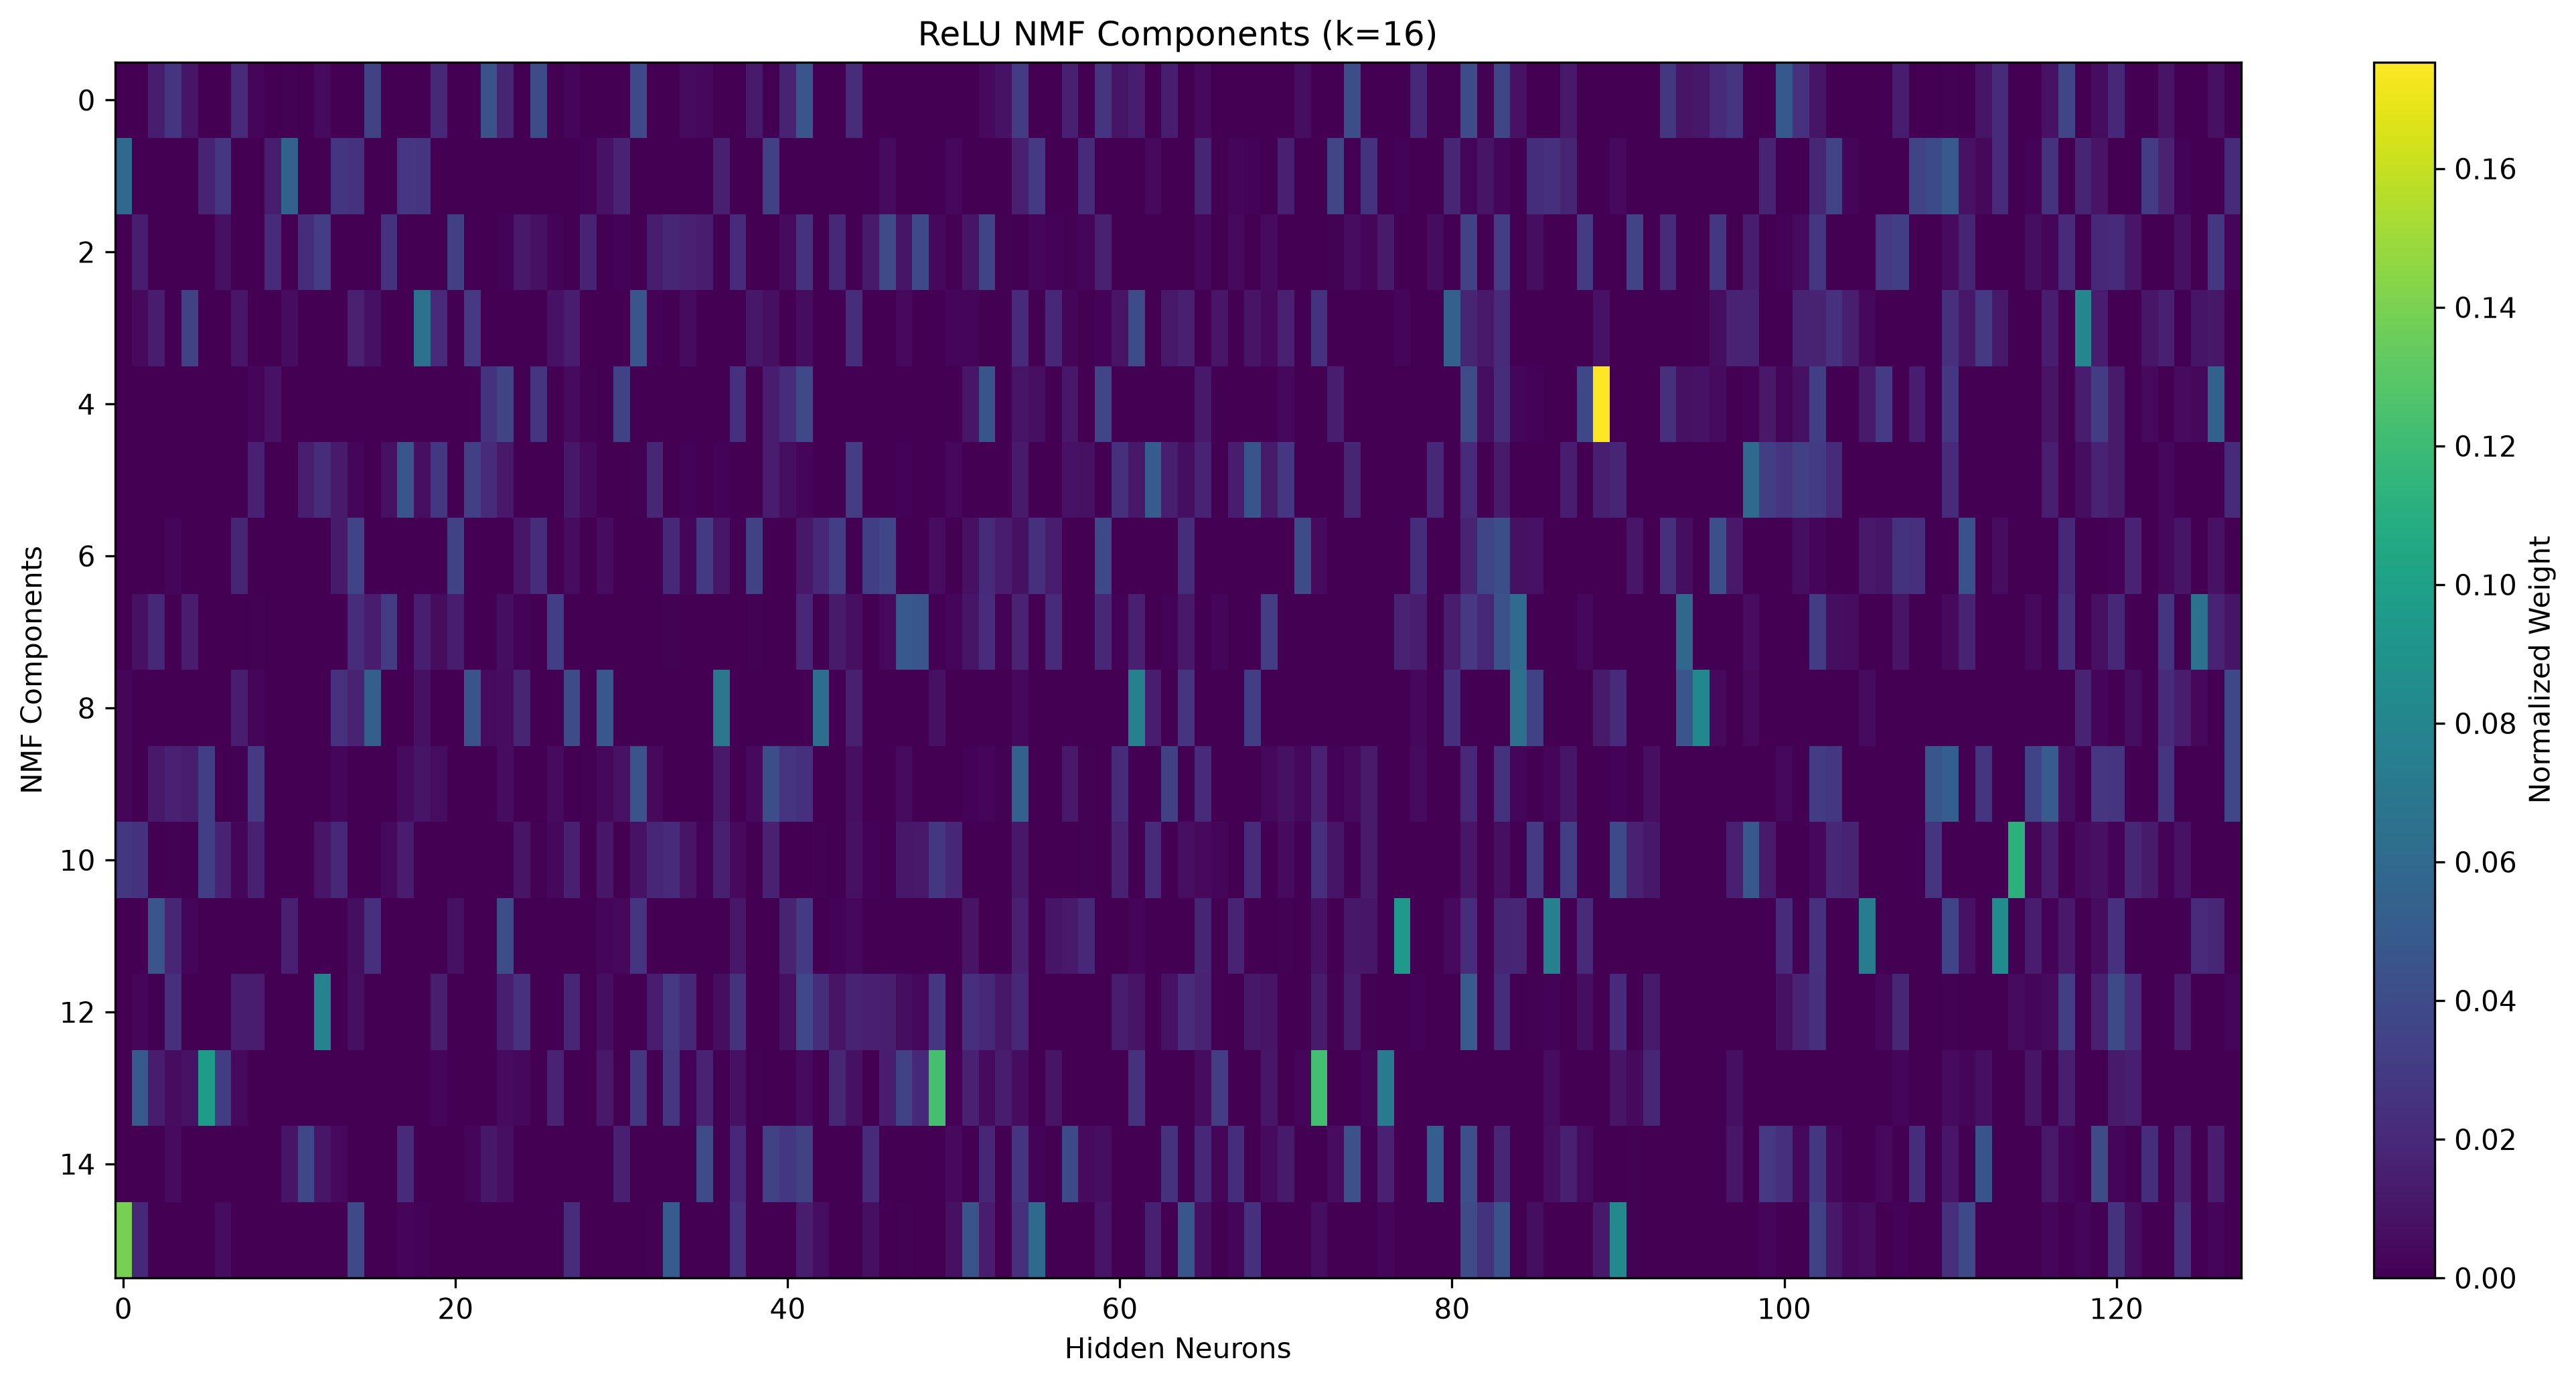
\includegraphics[width=\textwidth]{relu_nmf_components_k16.png}
  \caption{ReLU 激活矩阵 NMF 的成分矩阵 $H$（$k=16$，每行按行和归一化）。横轴为隐藏神经元编号，纵轴为成分编号。（\code{reports/figures/nmf/relu\_nmf\_components\_k16.png}）}
  \label{fig:comp}
\end{figure}

从图中可以看到，每个成分只在一部分神经元上有明显权重，其余位置接近零；不同成分的高权重位置各不相同。少数成分高度集中在个别神经元上，例如成分 4 在神经元 89 附近的归一化权重超过 0.16；另一些成分的权重分散在较多神经元上。定量来看，$k=16$ 时各成分的 Hoyer 稀疏度在 0.47 到 0.69 之间，平均为 0.563。因此，对 RQ3 的回答是肯定的：NMF 确实得到了一组在神经元空间中权重分布彼此不同、且相对集中的成分。

需要特别说明的是，图 \ref{fig:comp} 的横轴是神经元编号，而神经元没有天然的二维空间排列，相邻编号的神经元之间也没有特殊关系。因此，这张图不能像 Lee 与 Seung \cite{lee1999learning} 的人脸实验那样直接读成图像中的“局部部件”，更不能据此断定某个成分对应横线、竖线或弯钩等笔画。要建立这种对应，需要把成分映射回输入像素空间，而本项目尚未做这一步。

\subsection{NMF 类别关联}
\label{sec:class}

为了考察成分与数字类别的关系，图 \ref{fig:cls} 计算了每个类别的样本在各成分上的平均系数 $\bar w_{c,j}=\frac{1}{|\mathcal{I}_c|}\sum_{i\in\mathcal{I}_c}w_{ij}$，并对每一列（成分）除以其在 10 个类别上的最大值。这样，每列都有一个取值为 1 的“最强响应类别”。

\begin{figure}[htbp]
  \centering
  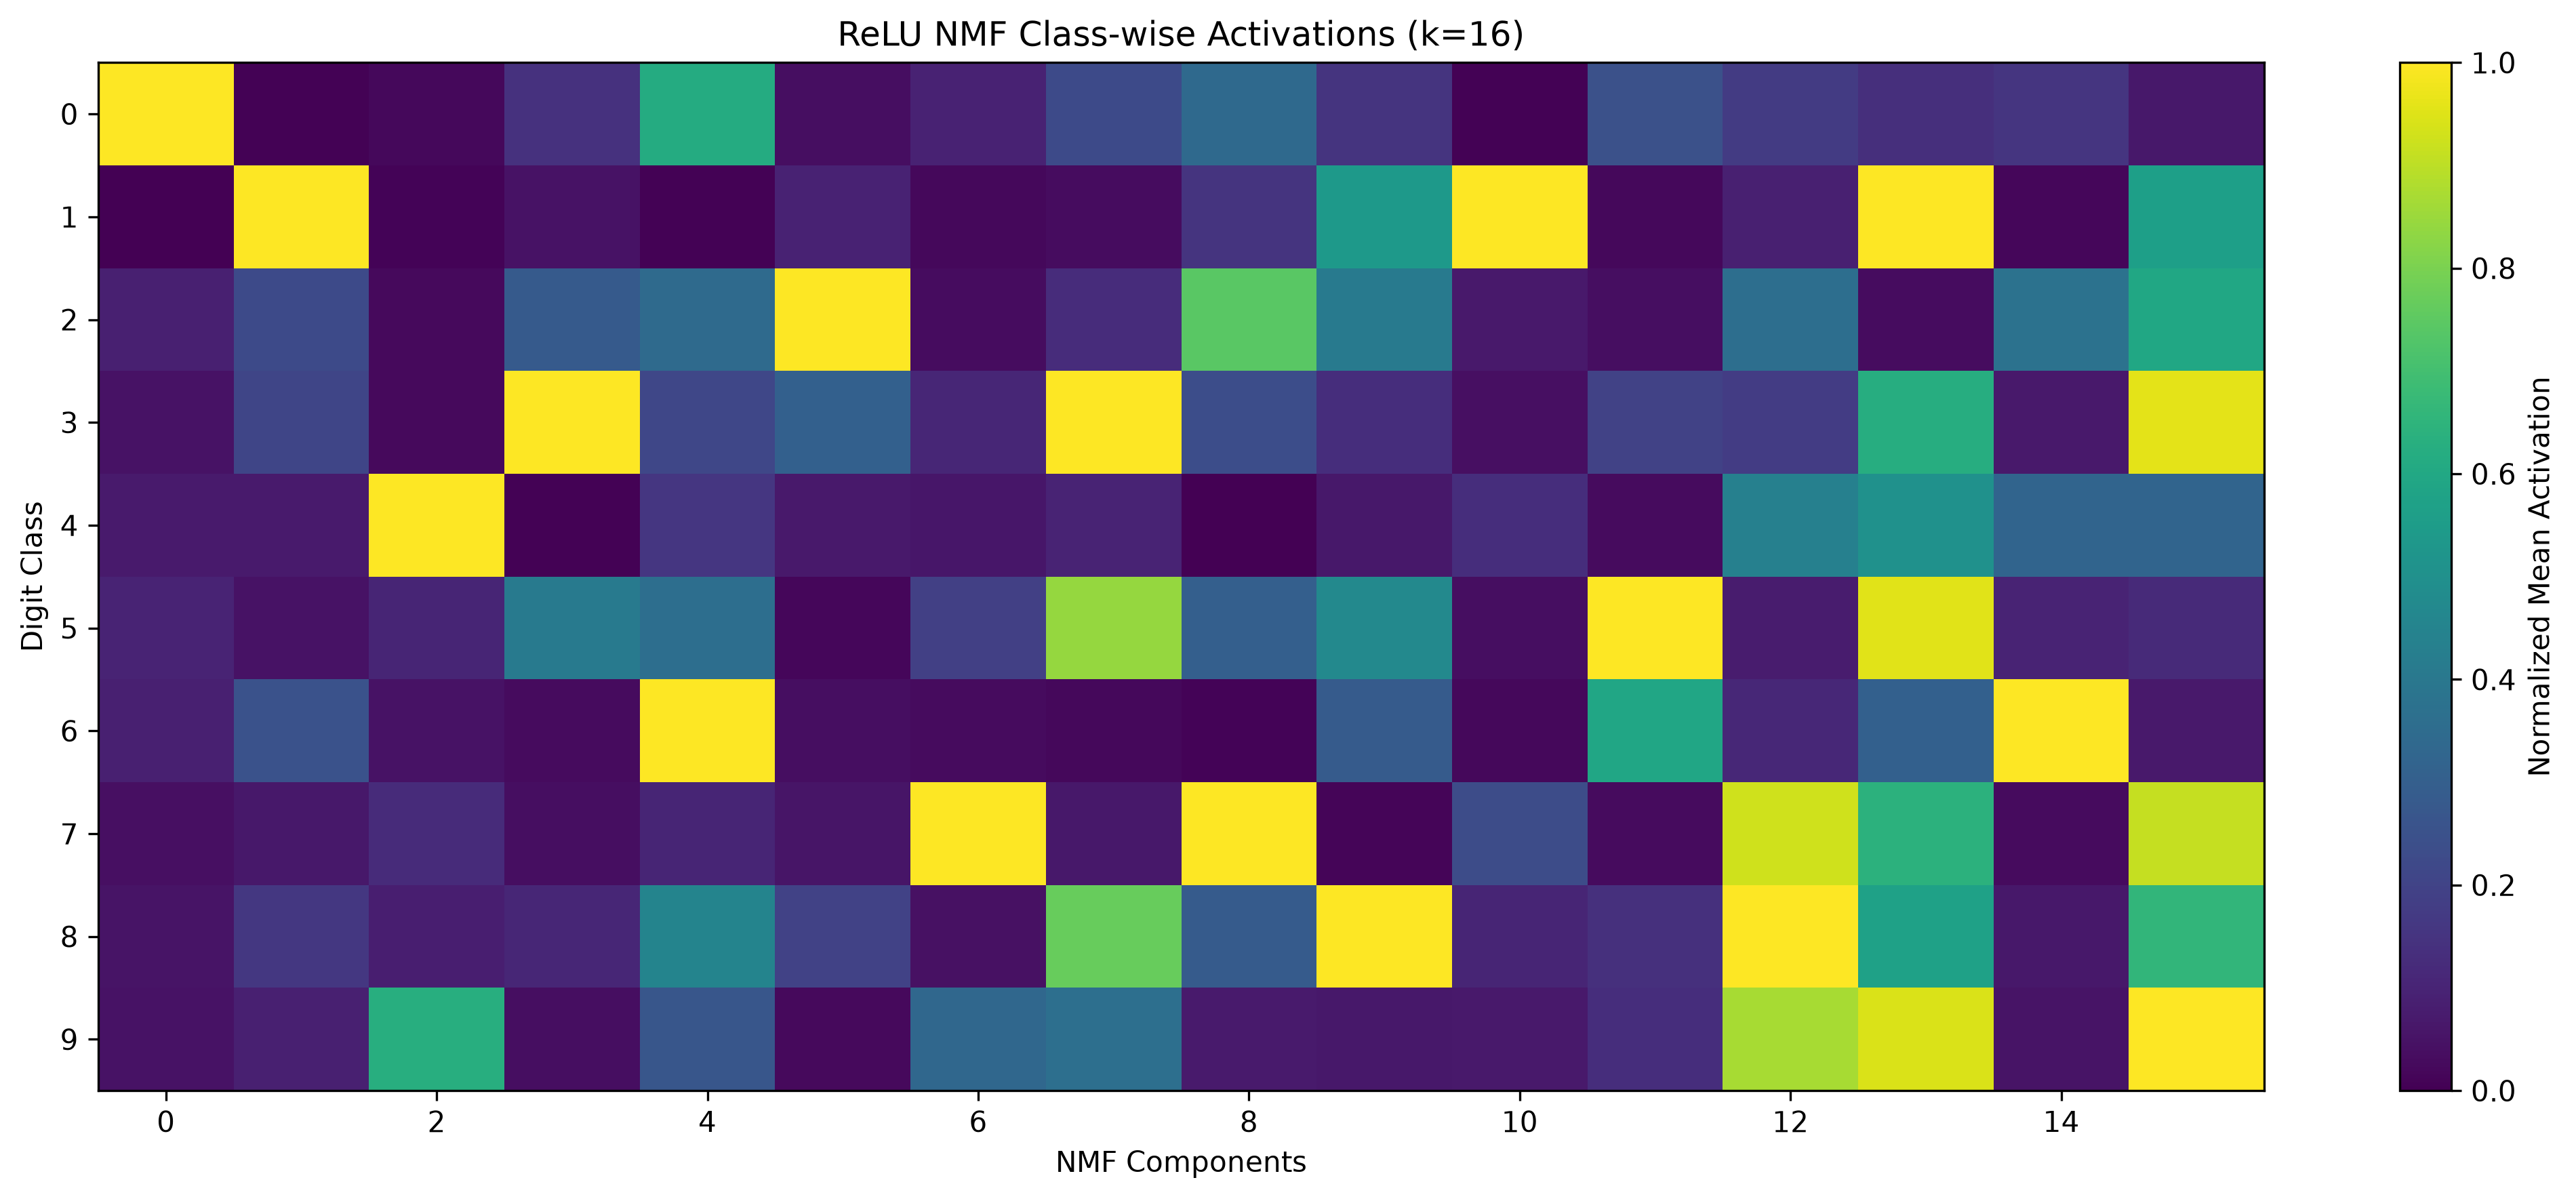
\includegraphics[width=\textwidth]{relu_nmf_class_activation_k16.png}
  \caption{ReLU NMF（$k=16$）各成分系数的类别均值，按列最大值归一化。纵轴为数字类别，横轴为成分编号。（\code{reports/figures/nmf/relu\_nmf\_class\_activation\_k16.png}）}
  \label{fig:cls}
\end{figure}

图 \ref{fig:cls} 显示出明显但不完全的类别关联。一方面，16 个成分的最强响应类别覆盖了全部 10 个数字，例如成分 0 主要对应数字 0，成分 2 对应数字 4，成分 5 对应数字 2。另一方面，许多成分同时对多个类别有较强响应：成分 12 在数字 7、8、9 上的归一化均值都在 0.85 以上，成分 13 在数字 1、5、9 上都接近 1。

为了量化这种“专属程度”，我们计算了每个成分最强类别与次强类别的均值之比（表 \ref{tab:clsratio}）。对 ReLU 而言，$k=16$ 时该比值的中位数为 1.77，16 个成分中只有 7 个超过 2。作为参照，我们也用同样方法计算了 Tanh Positive 的结果（仓库中没有对应的图），其中位数为 3.08，16 个成分中有 11 个超过 2。也就是说，按这一指标，\textbf{Tanh Positive 分解得到的成分与单一类别的关联反而更集中}。

\begin{table}[htbp]
  \centering
  \caption{NMF 成分的类别关联统计：最强类别均值与次强类别均值之比。由 \code{reports/nmf/} 中 $k=16,32$ 的 $W$ 与测试集标签计算。}
  \label{tab:clsratio}
  \begin{tabular}{l cc cc}
    \toprule
    & \multicolumn{2}{c}{$k=16$} & \multicolumn{2}{c}{$k=32$} \\
    \cmidrule(lr){2-3}\cmidrule(lr){4-5}
    & ReLU & Tanh Positive & ReLU & Tanh Positive \\
    \midrule
    比值中位数 & 1.77 & 3.08 & 1.67 & 1.76 \\
    比值 $>2$ 的成分数 & 7 / 16 & 11 / 16 & 11 / 32 & 14 / 32 \\
    覆盖的最强类别数 & 10 & 10 & 10 & 10 \\
    \bottomrule
  \end{tabular}
\end{table}

这些结果只说明成分系数与类别标签之间存在\emph{统计关联}。由于网络本身就是为分类而训练的，隐藏层表示与类别相关是意料之中的事；不能据此认为某个成分“专门识别”某个数字。

\subsection{ReLU 与 Tanh Positive 的定量比较}

图 \ref{fig:cmp} 把两组 NMF 的重构误差与成分稀疏度放在一起比较。原图的稀疏度部分只包含 $k=16$ 与 $k=32$；表 \ref{tab:hoyer} 补充了全部 8 个秩下的结果。

\begin{figure}[htbp]
  \centering
  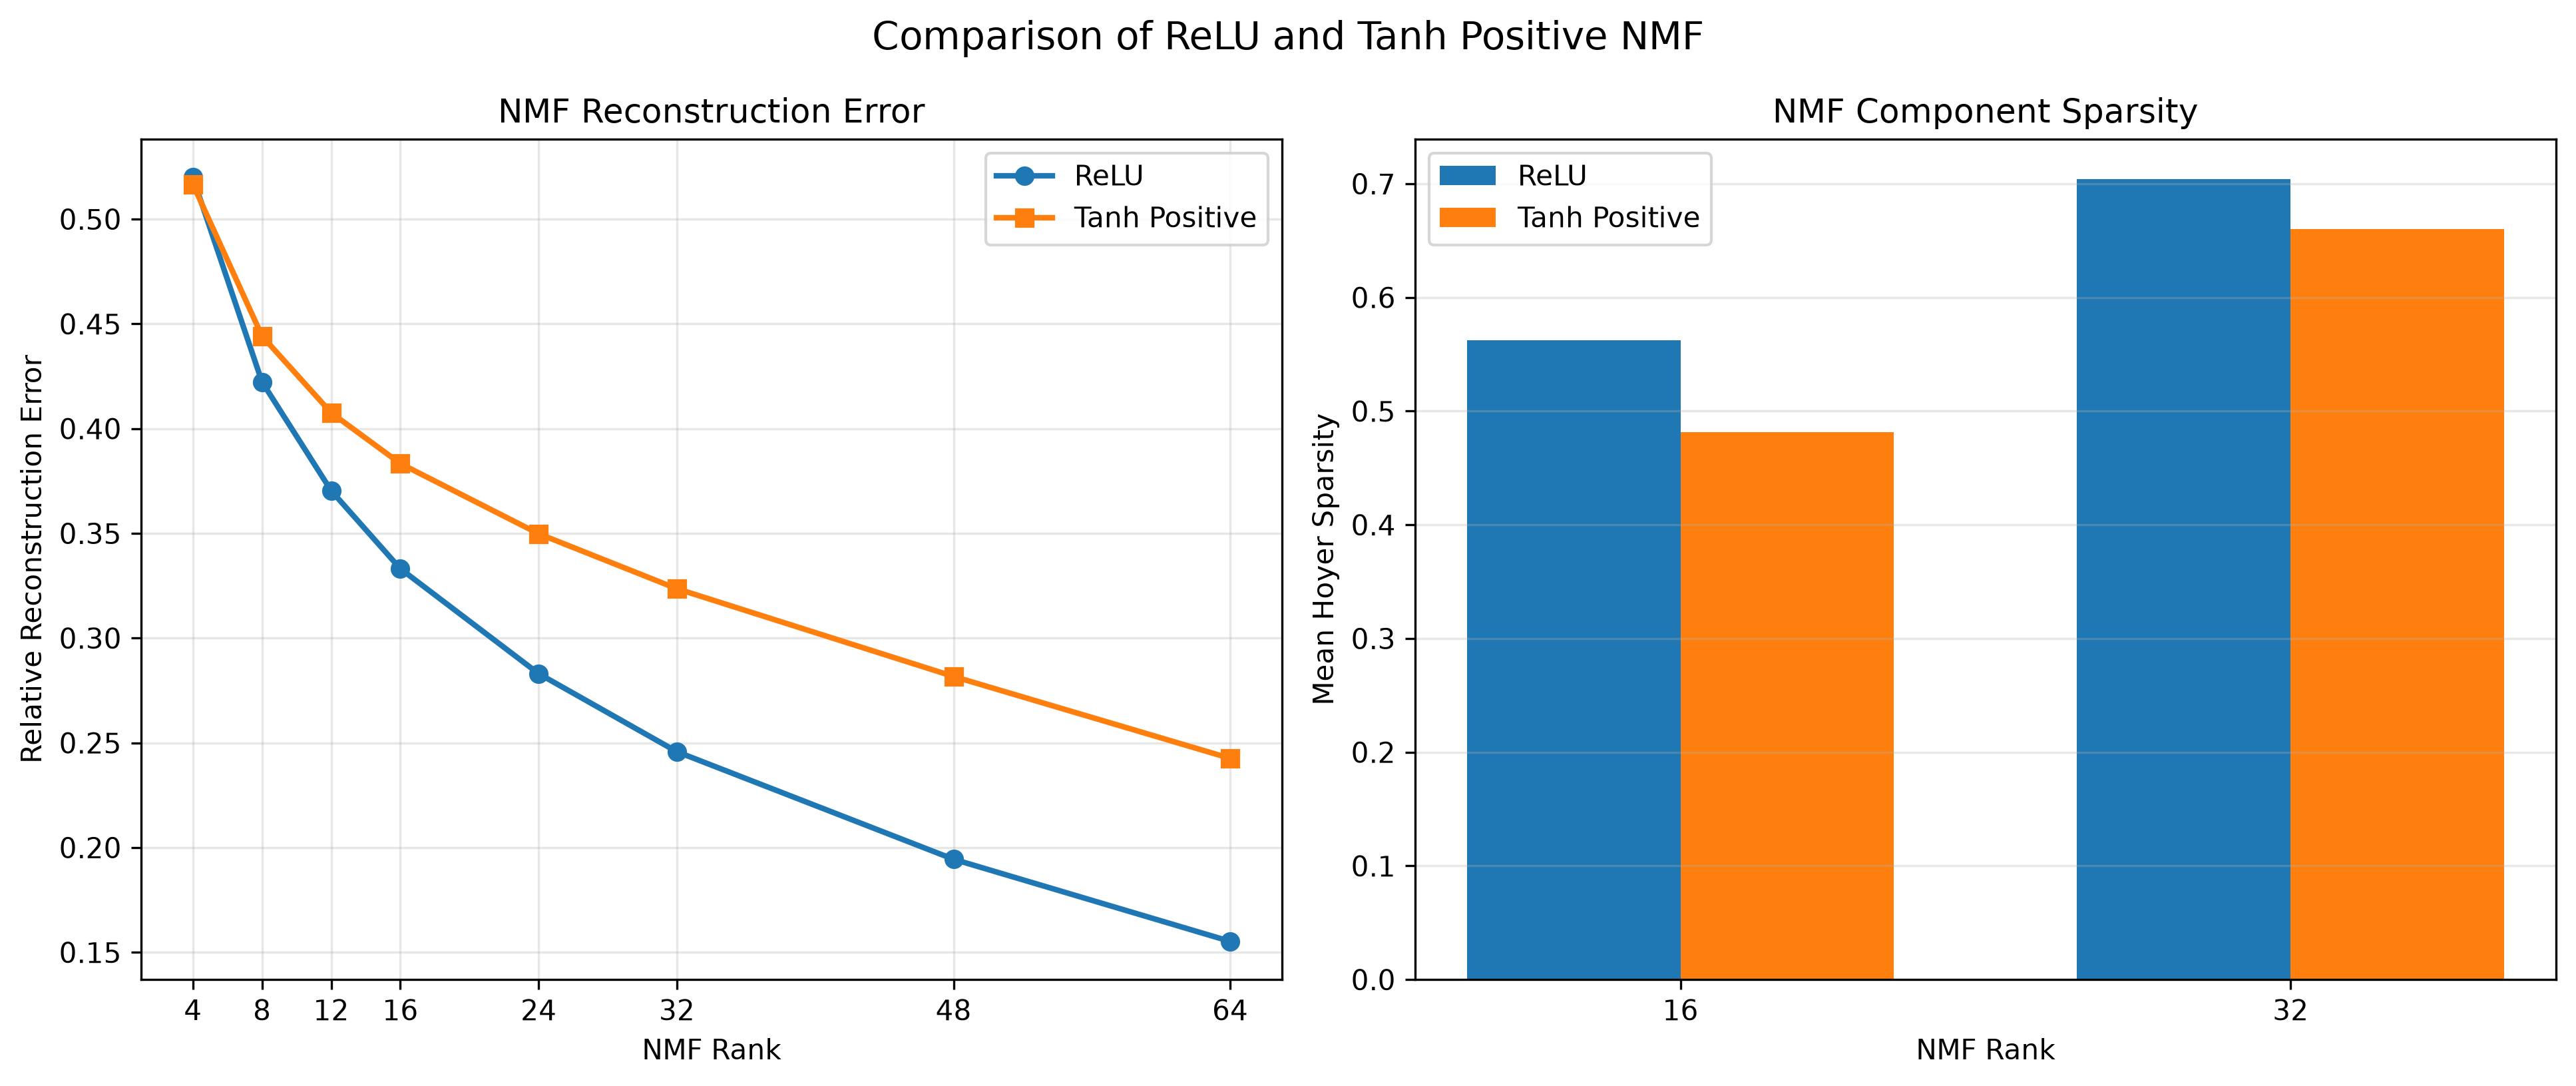
\includegraphics[width=\textwidth]{relu_tanh_nmf_comparison.png}
  \caption{ReLU 与 Tanh Positive 的 NMF 比较。左：相对重构误差随秩的变化；右：$k=16,32$ 时成分矩阵 $H$ 的平均 Hoyer 稀疏度。（\code{reports/figures/relu\_tanh\_nmf\_comparison.png}）}
  \label{fig:cmp}
\end{figure}

\begin{table}[htbp]
  \centering
  \caption{成分矩阵 $H$ 各行的平均 Hoyer 稀疏度。$k=32$ 的 ReLU 值与 \code{nmf\_component\_sparsity.json} 一致；其余由 \code{reports/nmf/*.npz} 计算。每列较大值加粗。}
  \label{tab:hoyer}
  \begin{tabular}{l cccccccc}
    \toprule
    $k$ & 4 & 8 & 12 & 16 & 24 & 32 & 48 & 64 \\
    \midrule
    \textcolor{relucol}{ReLU} & \textbf{0.367} & \textbf{0.435} & \textbf{0.508} & \textbf{0.563} & \textbf{0.635} & \textbf{0.704} & \textbf{0.783} & 0.841 \\
    \textcolor{tanhcol}{Tanh Positive} & 0.354 & 0.418 & 0.456 & 0.481 & 0.582 & 0.660 & 0.769 & \textbf{0.846} \\
    差值（ReLU $-$ Tanh$^+$） & 0.013 & 0.018 & 0.052 & 0.081 & 0.053 & 0.044 & 0.014 & $-0.005$ \\
    \bottomrule
  \end{tabular}
\end{table}

综合图 \ref{fig:cmp} 与表 \ref{tab:hoyer}，可以得到以下观察：
\begin{enumerate}
  \item 两组的 $H$ 稀疏度都随秩增大而单调上升：成分越多，每个成分需要覆盖的神经元越少。
  \item 在 $k=4$ 到 $48$ 的 7 个秩上，ReLU 的成分都更稀疏。差值在 $k=16$ 时最大（0.081），此后逐渐缩小。
  \item 在 $k=64$ 时，Tanh Positive 的成分稀疏度略高于 ReLU（0.846 对 0.841），两者已基本持平。
\end{enumerate}
因此，“ReLU 的 NMF 成分更集中”这一结论依赖于秩的选择：在中等秩范围内差异最明显，在很低或很高的秩下差异很小。而重构误差的优势（$k\ge8$）在整个范围内都成立。

% =============================================================
\section{讨论}

\subsection{实验结果说明了什么}

把第四章的结果放在一起，可以得到一个相对一致的图景：在本实验中，ReLU 网络的隐藏层激活\textbf{更容易被少量非负成分近似}，得到的成分在神经元维度上\textbf{也更集中}。对一个低秩非负近似来说，这两点并不矛盾：如果数据本身由若干相对独立、只涉及部分神经元的激活模式叠加而成，那么 NMF 既能用较少的成分重构它，得到的每个成分也只会覆盖少数神经元。ReLU 激活中“要么为零、要么明显为正”的特点（表 \ref{tab:act} 中精确零值与近零比例只差约 2 个百分点），与这种叠加结构在形式上是相容的。

但“相容”不等于“因果”。本实验只比较了两个具体的网络，无法区分以下几种解释：ReLU 的非负性本身导致了这种结构；ReLU 与 Tanh 的优化轨迹不同，导致学到的特征不同；或者问题主要出在 Tanh 一侧的预处理上（见下文）。这些解释都需要额外实验才能区分。

\subsection{比较的不对称性}

ReLU 与 Tanh Positive 的比较在设计上并不对称，这一点对解读结果很重要。$\Arelu$ 是 ReLU 网络\emph{实际使用}的完整表示，下一层的分类器看到的就是这个矩阵；$\Apos$ 则是人为截断后的矩阵，Tanh 网络的分类器同时依赖正值和负值。此外，Tanh 的大量激活饱和在 $\pm1$ 附近，截断后 $\Apos$ 中有很大一部分元素集中在 0 和接近 1 两个位置，带有一定的二值化特征。我们推测，这种由截断产生的、接近二值的结构，可能比 ReLU 激活中连续的正值更难用少量平滑的非负成分近似，从而贡献了 Tanh Positive 较高的重构误差。这一推测目前没有被直接检验。

\subsection{如何结合重构误差与 Hoyer 稀疏度}

重构误差和 $H$ 的稀疏度从两个方向描述同一个分解：前者回答“近似得好不好”，后者回答“成分是否集中”。二者通常存在权衡：成分越稀疏，表达能力越受限，近似可能越差。所以，单独看任何一个指标都不够。本实验中，ReLU 在 $k=8$ 到 $48$ 的范围内同时取得了更低的误差和更高的成分稀疏度，这比只在一个指标上占优更有说服力。不过到 $k=64$ 时，稀疏度的差异已经消失，提示这一“双重优势”只在中等秩下成立。

此外，$H$ 的稀疏度与原始激活的稀疏度是两件不同的事。原始激活的 Hoyer 稀疏度（表 \ref{tab:act}）描述的是每个样本有多少神经元活跃；$H$ 的 Hoyer 稀疏度（表 \ref{tab:hoyer}）描述的是每个成分涉及多少神经元。ReLU 在前者上远高于 Tanh（0.396 对 0.071），在后者上只是中等程度地领先，而且领先幅度随秩变化。原始激活更稀疏，并不意味着分解出的成分会同等程度地更稀疏。

\subsection{当前结果能否支持局部性与可解释性的假设}

本项目最初的直觉是：ReLU 的非负性可能使网络形成类似 NMF 的局部、可解释的表示，例如对应手写数字中的基本笔画。就目前的证据而言，这一假设\textbf{只得到了间接的、部分的支持}：
\begin{itemize}
  \item \textbf{支持的方面}：ReLU 激活具有大量精确零值；其 NMF 成分在神经元空间中更集中；成分与数字类别之间存在可辨认的关联。
  \item \textbf{不支持或无法判断的方面}：成分只定义在 128 个神经元组成的抽象空间中，没有映射回像素空间，因此无法判断它们是否对应笔画等视觉部件；单神经元的类别选择性上，Tanh 反而略高（图 \ref{fig:eta}）；在成分与类别的关联集中度上，Tanh Positive 也更高（表 \ref{tab:clsratio}）。
\end{itemize}
这些相反方向的证据提醒我们：对于“哪种表示更可解释”，不同的指标会给出不同的答案。

\subsection{为什么稀疏性不能等同于可解释性}

稀疏性是一个纯粹的数值性质，衡量的是非零元素或幅度的集中程度；可解释性则涉及人能否把某个成分与有意义的概念联系起来 \cite{doshivelez2017towards}。二者之间至少隔着三层距离。第一，一个只依赖少数神经元的成分，如果那些神经元本身的含义不清楚，这个成分照样难以解释。第二，Hoyer 稀疏度对缩放不变，也不关心\emph{哪些}元素非零，两个稀疏度相同的成分可能在语义上完全不同。第三，稀疏表示的经典成功案例，例如 Olshausen 与 Field \cite{olshausen1996emergence} 从自然图像中学到的局部、定向的感受野，以及 NMF 在人脸上得到的部件 \cite{lee1999learning}，都是\emph{在输入空间中}可视化后才显出意义的。本项目的成分停留在隐藏层空间，缺少这一步。因此，本文把较高的 Hoyer 稀疏度视为“表示更集中”的证据，而不把它视为“表示更可解释”的证据。

% =============================================================
\section{局限性}

\begin{enumerate}
  \item \textbf{Tanh 正值部分不等同于完整的 Tanh 表示。}$\Apos=\max(\Atanh,0)$ 丢弃了 52.16\% 的元素所携带的负值信息，使 ReLU 与 Tanh 的 NMF 比较在设计上不对称。更公平的做法可以是对正负拆分后的矩阵 $[\max(\Atanh,0),\ \max(-\Atanh,0)]$ 进行分解，或使用允许带符号数据的分解方法。
  \item \textbf{部分 NMF 配置未满足收敛条件。}16 组配置中有 7 组的迭代次数达到上限 500，且原始运行日志未保存。这些配置的误差与稀疏度可能尚未稳定，其中 Tanh Positive 受影响更多。
  \item \textbf{每种激活函数只有一次训练。}分类准确率、激活统计和 NMF 结果都来自单一随机种子，无法估计方差，也无法检验差异的统计显著性。NMF 本身也只用了一种初始化。
  \item \textbf{更高的稀疏性不必然意味着更强的可解释性。}如第五章所述，本文的成分没有映射回输入空间，也没有经过语义层面的评估；而在类别选择性等指标上，Tanh 并不弱于 ReLU。
  \item \textbf{结论受限于当前的模型与设置。}实验只涉及单隐藏层、128 个神经元的全连接网络，训练 5 个 epoch，使用 MNIST 数据集和一组固定的 NMF 超参数。对更深的网络、卷积网络或其他数据集，结论可能不同。
  \item \textbf{部分分析脚本与结果文件存在不一致。}例如 \code{analyze\_nmf\_class\_activation.py} 的输出文件名未正确格式化（生成了 \code{nmf\_class\_activation\_k\{k\}.npz}，$k=32$ 的结果覆盖了 $k=16$）；\code{plot\_relu\_tanh\_nmf\_comparison.py} 中的数值为手工录入。本文所用数值均已与原始 JSON 与 NPZ 文件逐一核对。
\end{enumerate}

% =============================================================
\section{结论}

本项目以 MNIST 为案例，探讨了神经网络的非负激活与非负矩阵分解之间的联系。我们训练了两个仅激活函数不同的单隐藏层网络，提取了它们在测试集上的隐藏层激活矩阵，比较了激活的分布与稀疏性，并在 8 个秩下对 ReLU 激活矩阵与 Tanh 激活矩阵的正值部分进行了 NMF。

在\textbf{实验事实}层面，本文观察到：
\begin{itemize}
  \item 两个网络的测试准确率分别为 97.13\% 与 96.83\%（单次训练）；
  \item ReLU 激活有 38.43\% 的精确零值，按样本的平均 Hoyer 稀疏度为 0.396；Tanh 激活呈 U 形分布，饱和明显；
  \item 两组 NMF 的相对重构误差都随秩单调下降；除 $k=4$ 外，ReLU 的误差都更低，且差距随秩增大；
  \item 在 $k\le48$ 时，ReLU 成分矩阵 $H$ 的平均 Hoyer 稀疏度更高，差值在 $k=16$ 时最大；到 $k=64$ 时两者基本持平；
  \item NMF 成分与数字类别之间存在统计关联，但多数成分并不专属于单一类别。
\end{itemize}

在\textbf{合理解释}层面，这些结果与“ReLU 激活具有较强的非负叠加结构”这一图景相容：ReLU 激活要么为零、要么明显为正，能被较少的、只涉及部分神经元的非负成分较好地近似。

在\textbf{仍待验证的假设}层面，本文的实验不足以说明 ReLU 表示比 Tanh 表示“更可解释”，也不足以说明 NMF 成分对应手写数字中的具体笔画。要检验这些假设，至少需要：多随机种子的重复实验；对 Tanh 采用保留符号信息的分解方式；确保 NMF 充分收敛；以及把成分映射回输入空间进行可视化与语义评估。

总之，本项目展示了如何用矩阵分解这一数值工具观察神经网络的内部表示，并给出了 ReLU 与 NMF 之间联系的一些具体数值证据。这种联系值得进一步研究，但不应被理解为二者在数学上等价，也不应被理解为更高的稀疏性足以证明更强的可解释性。

% =============================================================
% 参考文献样式由 gbt7714 宏包自动设置（GB/T 7714 顺序编码制）
\bibliography{references}

\end{document}
